\documentclass[journal,twoside,web]{ieeecolor}
\usepackage{generic}
\pdfminorversion=4

\usepackage{amsthm}
\usepackage{graphicx}
\usepackage{epsfig}
\usepackage{times}
\usepackage{amsmath}
\usepackage{amssymb}
\usepackage{cleveref}
\usepackage{subcaption,graphicx}
\usepackage{mathtools, cuted}
\usepackage{todonotes}
\usepackage{url}
\usepackage{color}
\usepackage{mathrsfs}
\usepackage{multirow}
\usepackage{caption}
\usepackage{subcaption}
\usepackage{cite}
\usepackage{wrapfig}
\usepackage{float}
\usepackage{mleftright}
\usepackage{nth}
\usepackage{dsfont}
\usepackage[normalem]{ulem}
\usepackage{tikz}
\usetikzlibrary{shapes,arrows}

\newtheorem{theorem}{Theorem}
\newtheorem{acknowledgement}[theorem]{Acknowledgement}
\newtheorem{algorithm}[theorem]{Algorithm}
\newtheorem{axiom}[theorem]{Axiom}
\newtheorem{assumption}[theorem]{Assumption}
\newtheorem{properties}[theorem]{Properties}
\newtheorem{case}[theorem]{Case}
\newtheorem{claim}[theorem]{Claim}
\newtheorem{conclusion}[theorem]{Conclusion}
\newtheorem{condition}[theorem]{Condition}
\newtheorem{conjecture}[theorem]{Conjecture}
\newtheorem{corollary}{Corollary}
\newtheorem{criterion}[theorem]{Criterion}
\newtheorem{con}[theorem]{Condition}
\newtheorem{definition}{Definition}
\newtheorem{exercise}[theorem]{Exercise}
\newtheorem{lemma}{Lemma}
\newtheorem{notation}[theorem]{Notation}
\newtheorem{problem}[theorem]{Problem}
\newtheorem{proposition}[theorem]{Proposition}
\newtheorem{solution}[theorem]{Solution}
\newtheorem{summary}[theorem]{Summary}
\newtheorem{remark}{Remark}
\newtheorem{example}[theorem]{Example}
\newtheorem{thm}{Theorem}
\newtheorem{cor}{Corollary}
\newtheorem{lem}{Lemma}
\newtheorem{prop}{Proposition}
\newtheorem{defn}{Definition}
\newtheorem{rem}{Remark}
\newtheorem{ass}{Assumption}

\DeclareMathOperator*{\infm}{inf}
\DeclareMathOperator*{\minimize}{minimize}
\DeclareMathOperator*{\maximize}{maximize}
\DeclareMathOperator*{\subjt}{subject \ to}
\DeclareMathOperator*{\sgn}{sign}
\DeclareMathOperator*{\argmin}{argmin}
\newcommand{\argmax}[1]{\underset{#1}{\operatorname{arg}\,\operatorname{max}}\;}
\newcommand{\pe}{\psi}
\newcommand{\R}{\mathbb{R}}
\newcommand{\trace}{\text{tr}}
\newcommand{\vecu}{{\bf u}}
\newcommand{\vece}{{\bf e}}
\newcommand{\vecc}{{\bf c}}
\newcommand{\dom}{\cal{D}}
\newcommand{\op}{\cal{L}}
\newcommand{\dop}{\cal{E}}
\newcommand{\x}{\textbf{x}}
\newcommand{\z}{\mathbb{Z}}
\newcommand{\real}{\mathbb{R}}
\newcommand{\p}{\partial}
\newcommand{\ps}{p^{\star}}
\newcommand{\PF}{\mathbb{P}}
\newcommand{\Tyx}{T_{y\rightarrow x}(p)}
\newcommand{\bi}{\begin{itemize}}
\newcommand{\ei}{\end{itemize}}
\newcommand{\bd}{\begin{displaymath}}
\newcommand{\ed}{\end{displaymath}}
\newcommand{\be}{\begin{align*}}
\newcommand{\ee}{\end{align*}}
\newcommand{\si}{\Sigma^{-1}}
\newcommand\norm[1]{\left\lVert#1\right\rVert}
\newcommand{\sub}[2]{(#1)_{(#2)}}

\title{\LARGE \bf Robust Optimization via Continuous-Time Dynamics}

\author{Keivan Ebrahimi, Nicola Elia, and Umesh Vaidya\\
\thanks{Financial support from the National Science Foundation grants CNS-1329915, ECCS-1150405, CIF-1220643, and ECCS-1810079 and from AFOSR grant FA95500119 are gratefully acknowledged. K. Ebrahimi is with the Department of Electrical \& Computer Engineering, Iowa State University, Ames, Iowa. U. Vaidya is with the Department of Mechanical Engineering, Clemson University, Clemson SC.  N. Elia is with the Department of Electrical and Computer Engineering, University of Minnesota, Twin Cities.
{\tt\small keivan@iastate.edu},
{\tt\small uvaidya@clemson.edu},
{\tt\small nelia@umn.edu}
}}

\begin{document}

\pagestyle{headings}
\setcounter{page}{1}
\pagenumbering{arabic}

\maketitle

\begin{abstract}
{\color{blue} We propose a continuous-time dynamical system approach for solving robust optimization problems without requiring explicit problem reformulations. Our ${\cal RO}$ dynamics treat uncertain variables as dynamical states and converge globally to optimal solutions for convex-concave robust optimization problems. Unlike existing methods that need complete a priori problem knowledge, our approach works with output feedback only and handles cases where robust counterparts cannot be derived. The method is suitable for real-time applications and provides guaranteed convergence without case-specific tuning. Numerical examples demonstrate effectiveness on problems ranging from quadratic programming to nonlinear optimization with complex uncertainty sets.}
\end{abstract}

\section{Introduction}

{\color{blue} With emerging applications that require solving real-time optimization problems in a reactive manner, this paper describes how interacting dynamical systems can find a robust solution for a broad class of robust optimization problems. This is particularly relevant in situations where physical systems must be steered towards optimal operating conditions, without prior knowledge of the functions to be optimized or the model of the uncertainty affecting the optimization. Recent advances in dynamical systems approaches to optimization \cite{aigner2023,zhang2023dynamics} and feedback-based methods \cite{zoranksg2023} have highlighted the importance of real-time robust solutions. Specifically, we propose a real-time approach to solving robust optimization problems, which has become increasingly important in recent years \cite{he2022}.} Optimization problems often involve various forms of uncertainty in the problem data. Two different approaches can be used: stochastic optimization, where uncertainty is treated as a random variable, or robust optimization (${\cal RO}$), where uncertainty is assumed to be deterministic and bounded. Unlike stochastic optimization, ${\cal RO}$ does not require any known probability distributions in the problem data. Instead, ${\cal RO}$ assumes that the uncertain data reside within a predefined uncertainty set, for which constraint violation cannot be tolerated. For more information on robust and stochastic optimization-based approaches, see \cite{bental2009}, \cite{bertsimas2011}, and the references therein. Early works on ${\cal RO}$ include \cite{soyster1976}, which considered robust linear optimization with ellipsoidal uncertainty sets, and \cite{falk1976}, which presented exact solutions of inexact linear programs as a simple case of ${\cal RO}$.

{\color{blue} The problem of robust linear programming was studied in \cite{bental1999}, while robust conic-quadratic optimization and robust semi-definite optimization were discussed in \cite{bental2002} and \cite{bental1998}, respectively. Refer to \cite{bertsimas2011} and \cite{beyer2007} for comprehensive surveys of ${\cal RO}$ problem solutions.

Recent developments in distributionally robust optimization (DRO) have bridged the gap between stochastic and robust approaches. \cite{aigner2023} developed data-driven DRO methods that adapt solutions over time as uncertainty sets shrink with incoming data. \cite{yang2023} introduced temporal correlation models for DRO under combined ambiguity. These advances enable more practical implementations where distributions evolve dynamically.

\cite{xu2009} and \cite{xu2010} showed that machine learning algorithms such as the norm-regularized support vector machine and the Lasso problem could be interpreted as ${\cal RO}$ problems. Recent work has further integrated robust optimization with machine learning: \cite{zoranksg2023} introduced zeroth-order optimization meeting human feedback for LLM improvement, while several papers focused on making machine learning problems robust against outliers, parameter uncertainties, and data perturbations through adversarial training \cite{lanckriet2003, bhattacharyya2004a, bhattacharyya2004b, trafalis2007, namkoong2016, sinha2018, esfandiari2019}.}

One of the main standard approaches for solving ${\cal RO}$ problems involves constructing a robust counterpart (RC) equivalent to the ${\cal RO}$ problem \cite{bental2009}. This widely used method essentially tries to find a deterministic equivalent to ${\cal RO}$ problem through a reformulation. In this sense, the practicality of robust programming depends on whether or not its RC is computationally tractable. An overview of different RO problems with tractable conjugates can be found in \cite{gorissen20152} Table 1 for some of which RC cannot be found.
The reformulation approach to solving the ${\cal RO}$ problem, which is often a challenging, albeit usually convex, optimization problem, has the deficiency of suffering from case-by-case scenarios depending on the specific form of the uncertainty constraint and the specific form of the uncertainty set. In other words, depending on how simple the uncertainty set looks and based on the optimization problem type (whether it is linear programming, quadratic programming, second-order cone programming, semi-definite programming, etc.), an RC is being calculated and provided at hand. These reformulations may be computationally more expensive than other approaches \cite{bertsimas2016}. Hence, the absence of a unified framework for solving a general class of ${\cal RO}$ problems without prior knowledge of the problem formulation is strongly felt.

{\color{blue} By calculating a concave conjugate of nonlinear constraint functions and supporting the function of uncertainty sets, \cite{bental20152} and \cite{gorissen20152} used the Fenchel duality to obtain a tractable RC for new classes of robust nonlinear optimization (RNO) problems. Recent work has extended these approaches: \cite{maxminmax2024} developed a novel max-min-max algorithm that operates directly on model functions through subgradient and projection oracles, enabling exploitation of problem structures without requiring explicit RC derivation. However, when no closed form is available for the convex conjugate function of an uncertainty set or convex/concave conjugates of a non-linear constraint, these approaches still cannot obtain the RC for many sets of nonlinear uncertainties and constraints.}

{\color{blue} An alternative randomized approach based on constraint sampling is an approximate probabilistic relaxation solution to ${\cal RO}$ problems as seen in \cite{calafiore2004} and \cite{calafiore2010} where a finite set of high-dimensional deterministic optimization problems obtained from sampling are solved. This approach does not require concavity of the constraint in the uncertain variable but due to the large number of required scenarios to approximate the stochasticity of these problems, the stochastic optimization involves formulating a large-scale scenario program, which is in general computationally demanding. To address this issue, \cite{rostampour2021} presented two methods using ADMM decomposition and soft communication schemes. More recently, \cite{drago2024} introduced the Drago algorithm, a stochastic primal-dual method achieving state-of-the-art linear convergence rates for strongly convex-strongly concave DRO problems with fine-grained dependency on primal and dual condition numbers.}

In another effort, \cite{bental2015} incorporated the min-max behavior of ${\cal RO}$ problems to solve them by an oracle-based approximate robust optimization algorithm based on oracle-based subgradient descent and interior point methods. The proposed algorithms find an approximate robust solution using a number of calls to an oracle that solves the original (non-robust) problem. However, the solution would be approximated with some predetermined accuracy, $\eta$, with the number of iterations growing to ${\cal O}(\frac{1}{\eta})$, as the algorithm approximates the RC by invoking the Oracle a polynomial number of times.
{\color{blue} Classical cutting-plane approaches such as \cite{mutapcic2009} treat ${\cal RO}$ problems as semi-infinite programming, iterating between optimization with fixed uncertainty values and posterior worst-case analysis. However, these methods have significant limitations when pessimization oracles are approximate.

\textbf{Modern developments in dynamical approaches:} Recent advances have substantially improved upon these classical approaches:
\begin{enumerate}
\item \textbf{Primal-dual dynamics:} \cite{timerescaling2023} analyzed time-rescaling of primal-dual dynamical systems with asymptotically vanishing damping, achieving fast convergence rates. \cite{pddamping2023} developed primal-dual damping algorithms whose continuous-time limits form second-order differential equations with proven linear convergence. \cite{meanfield2023} formulated stochastic programming as mean-field games where agents control primal-dual dynamics.
\item \textbf{First-order and zeroth-order methods:} \cite{nguyen2018} and \cite{he2022} developed efficient first-order algorithms reducing computational costs. \cite{chen2022} and \cite{zoranksg2023} introduced zeroth-order dynamics eliminating explicit gradient computations, with applications to RLHF and LLM optimization. \cite{zoro2023} combined zero-order robust optimization with real-time iteration schemes for efficient MPC implementation.
\item \textbf{Continuous-time optimization dynamics:} \cite{zhang2023dynamics} proposed projected primal-dual dynamical systems tracking optimizer trajectories for time-varying convex problems. \cite{onlineconvex2024} combined online convex optimization with robust MPC for controlling dynamical systems under uncertainty.
\item \textbf{Hardware implementations:} \cite{oscillator2024} established mathematical equivalence between coupled-oscillator machines and primal-dual Lagrange methods for combinatorial optimization.
\item \textbf{Distributionally robust advances:} \cite{aigner2023} and \cite{yang2023} developed adaptive DRO methods with shrinking ambiguity sets, while \cite{drago2024} achieved state-of-the-art convergence rates for DRO problems.
\end{enumerate}

While these state-of-the-art methods represent significant advances, they still require problem-specific adaptations and often lack the unified framework our dynamical system provides for general convex-concave robust optimization.}

{\color{blue} Robust optimization over time (ROOT) is another line of research combining robust optimization with dynamic optimization to model uncertainties from environmental changes. In these problems, robust solutions must adapt to major environmental changes. \cite{yazdani2023} provides a comprehensive review of ROOT papers. Recent work by \cite{aigner2023} on data-driven DRO over time demonstrates how robust solutions can adapt with shrinking ambiguity as more data becomes available, with solutions converging to stochastic optimization solutions. \cite{robusttodynamics2024} introduced robust-to-dynamics optimization combining mathematical programs with dynamic considerations, published in Mathematics of Operations Research.}

{\color{blue} Compared with existing ${\cal RO}$ methods, we point out that most existing algorithms are in a one-shot manner, requiring a priori knowledge of the uncertainty set model to formulate the optimization problem. Even recent advances in primal-dual dynamics \cite{timerescaling2023,pddamping2023} and distributionally robust methods \cite{aigner2023,drago2024} still require explicit problem formulation or distribution specifications. In contrast, our approach is independent of knowledge of the uncertainty set model as long as it is convex and the adversary variables enter concavely in the constraints and cost function. Unlike zeroth-order methods \cite{zoranksg2023,zoro2023} that rely on function evaluations or ranking oracles, our dynamics use only output feedback from the system. This fundamental difference opens up the possibility of having distributed real-time implementations of such systems in many settings where the uncertainty model and exact knowledge of the cost function and constraints are not available.}

In this paper, we provide the architecture of such a dynamical system that converges to the optimal robust solution for a large class of ${\cal RO}$ problems.

{\color{blue} \subsubsection{Main Contributions}
This paper makes the following key contributions that represent significant improvements over existing robust optimization methods:

\begin{enumerate}
\item \textbf{Model-free approach:} Unlike existing methods that require explicit knowledge of problem formulation, our approach works without a priori knowledge of the uncertainty set model, constraint functions, or objective function structure.
\item \textbf{Unified framework:} We provide a single dynamical system that can solve a general class of convex-concave robust optimization problems, eliminating the need for case-by-case reformulations required by robust counterpart methods.
\item \textbf{Novel dynamical system design:} We introduce the ${\cal RO}$ dynamics with a non-standard architecture that differs from classical primal-dual gradient methods, specifically designed to handle the min-max structure of robust optimization.
\item \textbf{Custom Lyapunov function:} We develop an unconventional Lyapunov function that enables global convergence analysis for our dynamical system, which does not follow from simple extensions of existing approaches.
\item \textbf{Real-time capability:} Our method provides continuous-time solutions suitable for real-time applications in dynamic environments, with demonstrated adaptability through numerical examples.
\item \textbf{Broader applicability:} Our approach can handle cases where robust counterparts cannot be derived or are computationally intractable, significantly expanding the class of solvable robust optimization problems.
\end{enumerate}}

{\color{blue} \subsubsection{Comparison with Existing Methods}
Table \ref{tab:comparison} provides a comprehensive comparison of our proposed ${\cal RO}$ dynamics with existing robust optimization approaches, highlighting the key advantages and limitations of each method.

\begin{table}[h]
\centering
\caption{Comparison of robust optimization approaches}
\label{tab:comparison}
\begin{tabular}{|l|c|c|c|c|}
\hline
\textbf{Method} & \textbf{Prior Knowledge} & \textbf{Real-time} & \textbf{General Applicability} & \textbf{Convergence} \\
\hline
Robust Counterpart & Full problem & No & Case-specific & Guaranteed \\
\cite{bental2009} & formulation & & reformulation & (when RC exists) \\
\hline
Scenario Sampling & Uncertainty & No & High computational & Probabilistic \\
\cite{calafiore2004} & distribution & & cost & approximation \\
\hline
Oracle-based & Problem structure & Limited & Requires oracles & $\mathcal{O}(1/\eta)$ \\
\cite{bental2015} & and oracles & & for subproblems & iterations \\
\hline
{\color{blue} Modern Oracle} & {\color{blue} First-order} & {\color{blue} Moderate} & {\color{blue} Gradient access} & {\color{blue} $\mathcal{O}(\log(1/\eta))$} \\
{\color{blue} \cite{he2022,chen2022}} & {\color{blue} methods} & & {\color{blue} required} & {\color{blue} for some cases} \\
\hline
{\color{blue} Primal-Dual} & {\color{blue} Problem} & {\color{blue} Yes} & {\color{blue} Continuous-time} & {\color{blue} Fast convergence} \\
{\color{blue} Dynamics \cite{timerescaling2023}} & {\color{blue} structure} & & {\color{blue} framework} & {\color{blue} with damping} \\
\hline
{\color{blue} DRO Methods} & {\color{blue} Distribution} & {\color{blue} Adaptive} & {\color{blue} Data-driven} & {\color{blue} Linear rate for} \\
{\color{blue} \cite{aigner2023,drago2024}} & {\color{blue} ambiguity} & & {\color{blue} approach} & {\color{blue} strongly convex} \\
\hline
Cutting Plane & Pessimization & No & Limited to cases & Depends on \\
\cite{mutapcic2009} & oracles & & with exact oracles & oracle quality \\
\hline
\textbf{RO Dynamics} & \textbf{Output feedback} & \textbf{Yes} & \textbf{Convex-concave} & \textbf{Global asymptotic} \\
\textbf{(This work)} & \textbf{only} & & \textbf{problems} & \textbf{stability} \\
\hline
\end{tabular}
\end{table}}

{\color{blue} Although our approach is inspired by classical work on primal-dual systems \cite{arrow1958,feijer2010} and recent advances in primal-dual dynamics \cite{timerescaling2023,pddamping2023,meanfield2023}, it presents significant architectural and convergence challenges described in this paper.} A key technical contribution is finding the right architecture of the dynamical system for which a non-standard Lyapunov function can help to prove global convergence to an optimal ${\cal RO}$ solution. The proposed continuous-time optimization system can solve a general class of ${\cal RO}$ problems where the cost function and the constraints are convex (concave) with respect to the decision variables (uncertain variables) and the uncertainty sets are convex\footnote{Preliminary convergence results for a special formulation appeared without proofs in \cite{ebrahimi2019continuous}. In this paper, we generalize the problem formulation and provide complete proofs, which are the core of our contributions.}. This class includes all the cases in \cite[~Table 1]{gorissen20152}.


The remainder of this paper is organized as follows. In Section \ref{sec_RO}, we present the problem statement of ${\cal RO}$ in a slightly generalized form. In Section \ref{section_saddle}, the characterization of saddle property and KKT optimality conditions along with the Lagrangian function for ${\cal RO}$ problem are provided. The main results on how to construct the ${\cal RO}$ dynamics is presented in Section \ref{section_pddynamics}. This section also includes the Lyapunov-based global convergence result. We then present simulation results in Section \ref{section_simulations} followed by conclusions in Section \ref{section_conclusions}.
Finally, detailed proofs are mentioned in the Appendix.

\section{Notations}\label{notations}

We define $i=0,\cdots,N$ as $i_{[N]}$, and $i=1,\cdots,N$ as $i^+_{[N]}$. In addition, $\left[\cdot\right]_\eta^+$ shows the positive projection defined as follows for the scalar-valued function $P$
\begin{align} \label{proj}
[P]_\eta^+:=\left\{\begin{array}{ccl}P&{\rm if}& P>0 \;{\rm or} \;\eta>0\\
0&{\rm otherwise}
\end{array}\right..
\end{align}
For vector-valued $P$, the projection is defined element-wise.

\section{Robust Optimization Problems}\label{sec_RO}
Given an objective $f_0(x)$ to optimize, subject to constraints $f_i(x,u_i) \leq 0$ with uncertain parameters, $\{u_i\}$, a classical robust optimization problem has the following form
$$
\begin{array}{ccc}
\mu&:=&\underset{x}{\min}\; f_0(x)\\
&&\text{s.t.}\;\;\;f_i(x,u_i)\leq 0,\;\;\;\; \forall \,u_i\in {\cal U}_i,\;\;\;i^+_{[N]}.
\end{array}
$$
where $x\in \real^n$ is a vector of decision variables, $f_0$ and $f_i$ are $\real^n \to \real$ functions, and the uncertainty parameters $u_i \in \real^{m_i}$ are assumed to take arbitrary values in certain convex compact uncertainty sets ${\cal U}_i \subseteq \real^{m_i}$.
The above problem is typically a semi-infinite optimization due to the cardinality of the ${\cal U}_i$. However, each robust constraint can be rewritten as a maximization problem as\footnote{{\color{blue}Since the uncertainty set is compact and the constraint functions are continuous, the supremum is attained within the set; therefore, we can replace "sup" with "max" in our formulation.}}
\begin{align}
\begin{array}{ccc}
\mu&:=&\underset{x}{\min}\; f_0(x)\\
&&\text{s.t.}\;\;\;\displaystyle\max_{{u_i\in \cal U}_i} f_i(x,u_i)\leq 0,\;\;\;\;i^+_{[N]}
\end{array}\;.\label{standardRO}
\end{align}

We consider a slight variation of (\ref{standardRO}), which takes the following under the assumptions stated below.
\begin{equation}\label{RO0}
\mathcal{RO}_0\left\{ \begin{array}{ccc}
&\mu:=\underset{x}{\min} \;\underset{u_0\in {\cal U}_0}{\max}\; f_0(x,u_0)\\
&\text{s.t.}\;\;\;\underset{u_i\in {\cal U}_i}{\max}\;\; f_i(x,u_i)\leq 0\;,\;i^+_{[N]},\\ \\
&{\cal U}_i:=\{u_ i\in \mathbb{R}^{m_i}\;:\;h_{ij}(u_i)\leq 0,\;\;j_{[K_i]}\}\;,\;i_{[N]}
\end{array}\right.
\end{equation}
{\color{blue} Here, $h_{ij}(u_i)$ represents the $j$-th constraint function defining the $i$-th uncertainty set ${\cal U}_i$, and $K_i$ denotes the total number of constraints that define the uncertainty set ${\cal U}_i$.} 

{\color{blue} \begin{remark}[Compactness of Uncertainty Sets Under Convex Assumptions]
The compactness requirement for uncertainty sets ${\cal U}_i$ is preserved under our convex assumptions for the following reasons:

\begin{enumerate}
\item \textbf{Convex constraint preservation:} Under Assumption \ref{assume1}, each $h_{ij}(u_i)$ is convex. The intersection of convex constraints $\{u_i : h_{ij}(u_i) \leq 0\}$ remains convex, preserving the geometric structure.

\item \textbf{Boundedness requirement:} For compactness, ${\cal U}_i$ must be bounded. This is typically ensured by including norm constraints (e.g., $\|u_i\| \leq \rho_i$) or box constraints as part of the $h_{ij}(u_i)$ system.

\item \textbf{Closedness from inequality constraints:} Since each $h_{ij}(u_i)$ is continuous and convex, the sublevel sets $\{u_i : h_{ij}(u_i) \leq 0\}$ are closed. The intersection of closed sets remains closed.

\item \textbf{Practical examples:} Common uncertainty sets like ellipsoids ($u_i^T Q_i u_i \leq 1$), polytopes ($A_i u_i \leq b_i$), and norm balls ($\|u_i\|_p \leq \rho_i$) all satisfy our convexity and compactness requirements.
\end{enumerate}

The combination of convexity, closedness, and boundedness ensures that ${\cal U}_i$ remains compact, which is essential for the existence of maximizers in the lower-level problems and the applicability of our dynamical system approach.
\end{remark}}

{\color{blue} \begin{remark}[Extension to Nonlinear Constraints in $u_i$]
While our current analysis focuses on constraints linear in the decision variables, the framework naturally extends to nonlinear constraints in the uncertainty parameters $u_i$ through the following considerations:

\begin{enumerate}
\item \textbf{Constraint structure preservation:} The uncertainty set definition ${\cal U}_i := \{u_i : h_{ij}(u_i) \leq 0\}$ already accommodates general nonlinear constraints. Our convexity assumption on $h_{ij}(u_i)$ ensures well-posed optimization problems.

\item \textbf{Dynamical system modification:} For nonlinear $h_{ij}(u_i)$, the ${\cal RO}$ dynamics (\ref{pd_dynamics}) remain structurally unchanged. The gradient terms $\nabla_{u_i} h_i(u_i)$ in the $v_i$ dynamics naturally handle the nonlinearity.

\item \textbf{Convergence preservation:} The Lyapunov analysis (Lemma \ref{monotonicity}) and convergence results (Theorem \ref{maintheorem}) extend to nonlinear uncertainty constraints as long as Assumption \ref{assume1} (convexity and smoothness) is maintained.

\item \textbf{Computational implications:} Nonlinear uncertainty constraints may increase computational complexity but do not fundamentally alter the theoretical foundations. Standard gradient-based methods can handle the resulting subproblems.

\item \textbf{Practical examples:} Nonlinear uncertainty sets commonly arise in engineering applications, such as energy constraints ($\sum_j u_{ij}^2 \leq P_i$), nonlinear budget constraints, and state-dependent uncertainty bounds.
\end{enumerate}

The key requirement is maintaining the convex-concave structure assumed in our analysis, which is naturally satisfied by many practical nonlinear uncertainty constraints.
\end{remark}}

The problem in (\ref{RO0}) reduces to the one in (\ref{standardRO}) when ${\cal U}_0$ is a singleton.
Following \cite{bental2009-2} and without loss of generality, we consider the ${\cal RO}$ problem dealing with constraint-wise uncertainties where each constraint $f_i$ is only a function of $u_i$.
The functions $f_i$ and $h_{ij}$ have scalar values with the following assumptions.

\begin{assumption}\label{assume1} The functions $h_{ij}(u_i)$ are convex in $u_i$ for $i_{[N]}$ and $j^+_{[K_i]}$.
The function $f_0(x,u_0)$ is strictly convex in $x$ for any $u_0\in {\cal U}_0$, and concave in $u_0$ for any $x$. Also, for $i^+_{[N]}$, $f_i(x,u_i)$ is convex in $x$ for fixed $u_i$ and concave in $u_i\in {\cal U}_i$, for fixed $x$.
Finally, the functions $f_i$ and $h_i$ $i_{[N]}$ are $C^1$ with local Lipschitz gradients.
\end{assumption}

{\color{blue} \begin{remark}[Justification of Assumption 1]
The convex-concave structure in Assumption 1 is fundamental for robust optimization and is satisfied by many practical problems. The convexity requirements ensure that the resulting optimization problems maintain desirable computational properties. This assumption can be extended in several directions:
\begin{enumerate}
\item The strict convexity in $x$ can be relaxed to mere convexity if uniqueness of the solution is not required.
\item The $C^1$ smoothness assumption can be extended to allow subgradient methods for non-smooth cases.
\item Many common uncertainty sets satisfy the convexity requirement, including ellipsoidal, polyhedral, and norm-bounded sets.
\end{enumerate}
In applications where the convex-concave structure does not naturally arise, it often can be induced through appropriate reformulation or approximation techniques.
\end{remark}}

\begin{assumption} \label{assume_feasible} Existence of optimal solutions and strong duality.

\begin{enumerate}
\item [A1] ${\cal RO}$ problem (\ref{RO}) is feasible. An optimal min-max solution $(x^\star,u^\star)$ exists and $\mu$ in the ${\cal RO}$ problem (\ref{RO}) is finite.
\item [A2] ${\color{blue}{\cal RO}$ problem satisfies the Slater constraint qualification, for both the upper level optimization and the lower level maximization problems}
 \cite{bental2009-2}, that is,
for all $i_{[N]}$ and all $j^+_{[K_i]}$, there exist $u_i \in {\cal U}_i$ such that $h_{ij}(u_i)<0,\;$  and
for $i^+_{[N]}$,  there exists $x \in \mathbb{R}^n$ such that, ${\cal F}_i(x)<0$\;.
\end{enumerate}
\end{assumption}
\begin{remark}
    It should be noted that the uncertainty is often parametrized affinely in ${\cal RO}$ problem; hence, the concavity property of the $f_i$ functions is automatically satisfied.
\end{remark}
{\color{blue} \begin{remark}[Justification of Assumption 2] \label{strong_duality_rem}
{\color{blue}Assumption [A2] (Slater constraint qualification) guarantees that the ${\cal RO}$ problem enjoys strong duality for upper and lower level optimization problems \cite[Section~5.2.3, 5.9.1]{boyd2004}.} While this assumption may appear restrictive, it can often be satisfied or relaxed in practice:
\begin{enumerate}
\item In many robust optimization applications, the uncertainty sets are designed with strict feasibility in mind (e.g., ellipsoidal sets with positive radius).
\item The assumption ensures that saddle point and optimal dual solutions exist \cite{bental2009-2}, which is crucial for our dynamical system approach.
\item For cases where Slater conditions are too restrictive, alternative constraint qualifications such as those discussed in \cite{jeyakumar2010} can be employed.
\item In practical implementations, the assumption can often be enforced by appropriate scaling or small perturbations of the constraint sets.
\end{enumerate}
\end{remark}}

Finally, we introduce the problem we consider in this paper, a slight generalization of ${\cal RO}_0$ in (\ref{RO0}).
\begin{equation}{\cal RO}\left\{\begin{array}{ccc}
&\mu:=\underset{x}{\min} \;\underset{u_0\in {\cal U}_0}{\max}\; f_0(x,u_0)+\displaystyle\sum_{i=1}^N c_i \underset{u_i\in {\cal U}_i}{\max}\;\; f_i(x,u_i)\label{RO}\\ \\
&\text{s.t.}\;\;\;\underset{u_i\in {\cal U}_i}{\max}\;\; f_i(x,u_i)\leq 0\;,\;i^+_{[N]},\\ \\
&{\cal U}_i:=\{u_ i\in \mathbb{R}^{m_i}\;:\;h_{ij}(u_i)\leq 0,\;\;j_{[K_i]}\}\;,\;i_{[N]}
\end{array}\right.
\end{equation}
where $c_i\geq 0$ for $i^+_{[N]}$. This setting can be seen as an elementary regularized version of more common formulations ${\cal RO}_0$ obtained for $c_i=0$, $i_{[N]}^+$.
The role of $c_i$ is further clarified in Remark \ref{active_inactive_constraint_rem}.

It is convenient to rewrite ${\cal RO}$ in the following form
\begin{align}
&\mu:=\underset{x}{\min} \; {\cal F}_0(x)+\sum_{i=1}^N c_i{\cal F}_i(x)\label{RO2}\\
&\;\;\text{s.t.}\;\;\;{\cal F}_i(x)\leq 0\;,\;i^+_{[N]}\;,\nonumber
\end{align}
where
\begin{equation}\label{G.eq}
{\cal F}_i(x):=\max_{u_i\in {\cal U}_i} f_i(x,u_i)\;,\; i_{[N]}\;.
\end{equation}
In this paper, we often call (\ref{G.eq}) as the "lower optimization problems", and the minimization in (\ref{RO2}) as the "upper optimization".

{\color{blue} \begin{remark}[Problem Formulation Clarifications]
To address potential confusion about our problem formulations, we clarify the relationships and motivations:

\textbf{Classical vs. Our Formulation:} The classical robust optimization problem (\ref{standardRO}) has constraints $\max_{u_i \in {\cal U}_i} f_i(x,u_i) \leq 0$. Our formulation (\ref{RO}) adds the $c_i$ terms in the objective, creating a regularized version that provides several advantages:

\begin{enumerate}
\item \textbf{Inactive constraint handling:} When robust constraints are inactive ($\lambda_i = 0$), the $c_i$ terms prevent the dynamics from becoming singular and ensure convergence.
\item \textbf{Computational benefits:} The regularization improves numerical stability and enables unified analysis for both active and inactive constraints.
\item \textbf{Flexibility:} The formulation naturally recovers the classical case when $c_i \to 0$ as constraints become active.
\end{enumerate}

\textbf{Non-smoothness consideration:} While taking the maximum in (\ref{standardRO}) introduces non-smoothness compared to individual constraints, this is fundamental to robust optimization. Our dynamical approach handles this non-smoothness naturally through the min-max structure, avoiding the need for explicit smoothing techniques.

\textbf{Role of $c_i$ terms:} Rather than using alternative multipliers $\gamma_i := c_i + \lambda_i$, our approach treats $c_i$ as regularization parameters and $\lambda_i$ as proper dual variables. This separation maintains the physical interpretation of dual variables while providing mathematical convenience.

{\color{blue} \textbf{Why separate $c_i$ and $\lambda_i$ instead of using $\gamma_i$:} The suggestion to use $\gamma_i := c_i + \lambda_i$ would mathematically simplify some expressions, but our separation provides several theoretical and practical advantages:
\begin{enumerate}
\item \textbf{Dual variable interpretation:} The $\lambda_i$ terms retain their classical interpretation as shadow prices of constraints, allowing standard economic interpretation of optimality conditions.
\item \textbf{Regularization control:} The $c_i$ parameters can be chosen independently of the optimization process to control numerical stability and convergence behavior.
\item \textbf{Asymptotic recovery:} As $c_i \to 0$, the formulation naturally converges to the classical robust optimization problem, while maintaining well-defined dynamics throughout the transition.
\item \textbf{Convergence analysis:} The separation enables the construction of our Lyapunov function (\ref{Lya_function}) with coefficients $(c_i + \lambda_i^*)$ that have clear geometric meaning.
\end{enumerate}

\textbf{Non-smoothness from maximum operations:} The max operators in formulation (\ref{standardRO}) create fundamental non-smoothness that affects both problem structure and solution methods:
\begin{enumerate}
\item \textbf{Source of non-smoothness:} Each constraint $\max_{u_i \in {\cal U}_i} f_i(x,u_i) \leq 0$ defines a non-smooth function in $x$, as the maximum operation is non-differentiable when multiple $u_i$ values achieve the maximum.
\item \textbf{Traditional challenges:} Standard gradient-based methods fail because gradients may not exist, and subgradient methods require specialized analysis for convergence guarantees.
\item \textbf{Our approach advantages:} The dynamical system formulation naturally handles non-smoothness through:
   \begin{itemize}
   \item \textbf{Dual decomposition:} The Lagrangian structure decomposes the non-smooth max problem into smooth subproblems.
   \item \textbf{Projection operators:} The $[\cdot]^+$ projections in dynamics (\ref{pd_dynamics}) handle constraint boundaries without requiring explicit smoothness.
   \item \textbf{Saddle point convergence:} The min-max structure converges to the correct solution despite non-smoothness in individual constraint functions.
   \end{itemize}
\item \textbf{Theoretical handling:} Our convergence analysis (Theorem \ref{maintheorem}) demonstrates that the continuous-time dynamics overcome non-smoothness through the inherent averaging effect of differential equations, providing global convergence guarantees that discrete methods cannot achieve.
\end{enumerate}}
\end{remark}}

As already mentioned, our formulation includes the typical robust optimization formulation ${\cal RO}_0$
\begin{equation}
\begin{array}{lcc}
\mu=&\;\displaystyle\min_x f_0(x)\\
s.t.&\; {\cal F}_i(x)\leq 0,\;\;i^+_{[N]}
\end{array}\;,
\label{RO3}
\end{equation}
or the form below that is popular in the machine learning context \cite{rafique2022,zhang2021}
\begin{equation}
\mu=\;\displaystyle\min_x\max_{u\in {\cal U}} f_0(x,u)\;.
\end{equation}
We finally introduce the following assumption valid for most of this paper.

\begin{assumption} \label{assume_c>0}
\begin{enumerate}
\item [A3] $c_i > 0$ for $i^+_{[N]}$.
\end{enumerate}
\end{assumption}


{\color{blue} \begin{remark}[Justification and Relaxation of Assumption 3] \label{active_inactive_constraint_rem}
Assumption [A3] requiring $c_i > 0$ serves important technical and practical purposes, though it can be relaxed under certain conditions:

\textbf{Technical justification:} The positive $c_i$ terms provide regularization that ensures convergence when robust constraints are inactive, preventing the dynamics from becoming singular.

\textbf{Practical implications:} In real applications, the $c_i$ parameters can be chosen as:
\begin{enumerate}
\item Very small values (e.g., $c_i = 10^{-6}$) that don't significantly affect the solution but ensure numerical stability.
\item Adaptive values that decrease as the algorithm converges, eventually approaching zero.
\item Zero values when all constraints are known to be active at the optimal solution.
\end{enumerate}

\textbf{When assumption can be relaxed:} The constraint $c_i > 0$ can be relaxed to $c_i \geq 0$ under the stronger assumption that all robust constraints are active at the optimum. This recovers the classical robust optimization formulation (\ref{RO3}) as a special case.

\textbf{Empirical selection strategies:} In practice, $c_i$ values can be selected based on problem scaling, constraint sensitivity analysis, or through adaptive algorithms that monitor constraint activity during the optimization process.

\textbf{Extension to proximal methods:} For problems where strict complementarity assumptions may be too strong, our framework can be extended to include proximal regularization terms. Specifically, one can consider the modified formulation:
\begin{align}
\min_x \; {\cal F}_0(x) + \frac{\rho}{2}\|x - x_{ref}\|^2 + \sum_{i=1}^N c_i {\cal F}_i(x)
\end{align}
where $\rho > 0$ and $x_{ref}$ is a reference point. This proximal term helps recover strong monotonicity at saddle points and provides convergence guarantees even when some robust constraints are inactive, addressing limitations in scenarios with structural regularity requirements.
\end{remark}}

\subsection{Robust feasible solution and robust counterpart}
A meaningful solution to ${\cal RO}$ problem (\ref{RO}) has to be immune against the uncertainties in the sense that the solution vector $x$ should satisfy the constraints for all $u_i$'s within the uncertainty sets\footnote{Similar to what is meant by feasibility in Robust Control \cite{zhou1995}.}. Such vector $x$ is called a robust feasible solution (RFS). One approach to solving the problem (\ref{RO}) is to try to compute (\ref{G.eq}) in closed form.

For various important combinations of constraint functions $f_i$ and uncertainty sets ${\cal U}_i$, ($i>0$) it is possible to obtain an explicit convex function ${\cal F}_i$ \cite{bental2009}. A classical example is when $f_i$ is linear in $x$ for fixed $u_i$ and linear in $u_i$ for fixed $x$, while ${\cal U}_i$ is an ellipsoidal set.
Then, ${\cal F}_i$ can be easily derived as an explicit second-order conic function.
In this case, ${\cal RO}$ problem (\ref{RO}) becomes a nominal optimization problem (not affected by uncertainty) known as the explicit {\color{blue}Robust Counterpart (RC)}:
\begin{align} \label{rc}
\displaystyle \min_{{\cal F}_i(x)\leq 0} f_0(x)\;.
\end{align}
As shown in \cite{bental2009-2}, the RC is always a convex optimization problem under Assumption \ref{assume1}. While the RC is known for important classes of problems as described in \cite{bertsimas2011}, this approach requires problem-specific derivations; moreover, RC is generally difficult to find (See Section \ref{section_simulations} for an example). Instead, our proposed approach has a dynamical system that simultaneously finds the best RFS and the worst parameters $u_i$' s, independently of the specifics of the constraint functions and the uncertainty sets.


\section{Duality, KKT conditions and saddle property} \label{section_saddle}
The basic idea of this paper is to combine the usually separated and nested optimization (\ref{RO2}) and (\ref{G.eq}) into one Lagrangian optimization.

To derive the Lagrangian function for ${\cal RO}$ problem (\ref{RO}), we introduce Lagrange multipliers $\lambda_i\geq 0$ for $i^+_{[N]}$, and let $\lambda=(\lambda_1,\lambda_2,\cdots,\lambda_N)^\top \in \mathbb{R}_+^N$ where the non-negative orthant of $\mathbb{R}^N$ is denoted by $\mathbb{R}_+^N$. Note that $\mu$ in ${\cal RO}$ problem (\ref{RO}) can be written in short-hand notation  as follows
\begin{align}
\mu=&\;\underset{x}{\min}\;\underset{\lambda\geq 0}{\max}\; {\cal F}_0(x)+\sum_{i=1}^N (c_i+\lambda_i) \; {\cal F}_i(x)\;,
 \label{upper_ro}
\end{align}
where ${\cal F}_i(x)$ is given by (\ref{G.eq}).
 By introducing Lagrange multipliers $v_{ij} \geq 0$ for the maximization problem in (\ref{G.eq}) and defining
\begin{align*}
v_i:=(v_{i1},\cdots, v_{iK_i})^\top \in \mathbb{R}_+^{K_i},\;h_i:=(h_{i1},\cdots, h_{iK_i})^\top\;,\nonumber
\end{align*}
the lower level strong duality (according to Assumption \ref{assume_feasible}) yields
\begin{align} \label{lower_ro}
{\cal F}_i(x)=\underset{u_i\in \mathbb{R}^{m_i}}{\max}\;\underset{v_{i}\geq 0}{\min}\;f_i(x,u_i)-v_i^\top h_{i}(u_i)\;.
\end{align}

Defining the Lagrangian $\tilde {\cal L}_i:\mathbb{R}^n \times \mathbb{R}^{m_i} \times \mathbb{R}^{K_i} \rightarrow \mathbb{R}$ for the lower level maximization problem (\ref{lower_ro}) as
\begin{align} \label{lower_lag}
\tilde {\cal L}_i(x,u_i,v_i):=f_i(x,u_i)-v_i^\top h_{i}(u_i),\;i^+_{[N]},
\end{align}
and
\begin{align} \label{upper_lag}
\tilde {\cal L}_0(x,u_0,v_0):=f_0(x,u_0)-v_0^\top h_{0}(u_0)\;.
\end{align}
In the optimization problem (\ref{upper_ro}), $\mu$ can be written as
\begin{align} \label{main_RO_eq}
\mu=\underset{x}{\min}&\;\underset{\lambda\geq 0}{\max}\;\underset{u_0}{\max}\;\underset{v_0\geq 0}{\min}\;\; \tilde{\cal L}_0(x,u_0,v_0)\\
&+\sum_{i=1}^N (c_i+\lambda_i)\; \underset{u_i}{\max}\;\underset{v_{i}\geq 0}{\min}\;\;\tilde {\cal L}_i(x,u_i,v_i)\;\nonumber.
\end{align}
or combining the independent maximizations and minimizations, and collecting the variables, we have
\begin{align}\label{main_RO2_eq}
\mu=&\min_{x}\max_{\lambda\geq 0}\max_{u}\min_{v\geq 0} \\
&\big(\tilde{\cal L}_0(x,u_0,v_0)+\sum_{i=1}^N (c_i+\lambda_i) \; \tilde {\cal L}_i(x,u_i,v_i)\big)\;.\nonumber
\end{align}
Hence, we showed the equivalence of (\ref{RO}) and (\ref{main_RO_eq}).
The complete Lagrangian ${\cal L}(x,\lambda,u,v)$ for ${\cal RO}$ problem is derived as
\begin{align}
{\cal L}(x,\lambda,u,v)&\;:=\;f_0(x,u_0)-v_0^\top h_0(x,u_0)\nonumber\\
&+\sum_{i=1}^N (c_i+\lambda_i)\big(f_i(x,u_i)-v_i^\top h_i(x,u_i)\big)\;,
\label{lag}
\end{align}
which leads to
\begin{align*}
\mu=\min_{x}\max_{\lambda\geq 0}\max_{u}\min_{v\geq 0}\;{\cal L}(x,\lambda,u,v)\;.
\end{align*}
From Remark \ref{strong_duality_rem}, strong duality holds for both upper and lower optimizations. Thus, we can switch the order of max and min as follows
\begin{equation}\label{dual.eq}
\mu=\max_{\lambda\geq 0}\;\min_{x}\min_{v\geq 0} \max_{u}\;{\cal L}(x,\lambda,u,v)\;.
\end{equation}

\begin{definition} \label{optimal_ro}
We denote an optimal solution of (\ref{dual.eq}), $z^\star:=(x^\star,\lambda^\star,u^\star,v^\star)$, as an {\color{blue}``optimal ${\cal RO}$ solution''}, where $(x^\star, u^\star)$ is an optimal solution for (\ref{RO}), and $(\lambda^\star, v^\star)$ are optimal values for the corresponding dual variables according to the principles in \cite[Section~5.9.1]{boyd2004}.
\end{definition}

\subsection{KKT optimality conditions}

{\color{blue} \begin{remark}[KKT Conditions for Robust Optimization]
The KKT conditions presented below follow the standard KKT framework from \cite{boyd2004} but are specialized for our robust optimization formulation (\ref{RO}). The key distinctions from standard optimization are:

\begin{enumerate}
\item \textbf{Bi-level structure:} The conditions simultaneously address both the upper optimization over $x$ and the lower maximizations over $u_i$, requiring coordination between dual variables $\lambda_i$ and $v_{ij}$.

\item \textbf{Regularization terms:} The $(c_i + \lambda_i)$ terms in (\ref{kkt1}) reflect our regularized formulation, where $c_i$ provides stability when constraints are inactive.

\item \textbf{Nested complementary slackness:} Conditions (\ref{kkt3}) and (\ref{kkt4}) enforce complementary slackness at both levels of the optimization hierarchy.

\item \textbf{Saddle point characterization:} These KKT conditions are equivalent to the saddle point conditions for the unified Lagrangian (\ref{lag}), enabling our dynamical system approach.
\end{enumerate}

While the mathematical form follows standard KKT theory, the interpretation and application to robust optimization's nested structure is specific to our approach.
\end{remark}}

As strong duality holds for ${\cal RO}$ problem, any optimal solution, $z^\star=(x^\star,\lambda^\star,u^\star,v^\star)$, satisfies the following Karush-Kuhn-Tucker (KKT) conditions, and vice-versa \cite{boyd2004}
\begin{align}
&\nabla_x f_0(x^\star,u_0^\star)+  \sum_{i=1}^N(c_i+\lambda^\star_i) \nabla_x f_i(x^\star,u_i^\star)=0,\label{kkt1}\\
&\nabla_{u_i} f_i(x^\star,u_i^\star)-{v_i^\star}^\top \nabla_{u_i} h_i(u_i^\star)=0,\; i_ {[N]},\label{kkt2}\\
&\;v_{ij}^\star\geq 0,\; h_{ij}(u_i^\star)\leq 0,\;v_{ij}^\star h_{ij}(u_i^\star)=0,\;  j^+_{[K_i]}, i_{[N]} \label{kkt3}\\
&\lambda_i^\star\geq 0,\;f_{i}(x^\star,u_i^\star)\leq 0,\;\lambda_i^\star f_{i}(x^\star,u_i^\star)=0,\;i^+_{[N]} \label{kkt4}
\end{align}
where $\nabla_x f$ is the notation for the gradient of a function $f$ w.r.t. $x$.

\subsection{{\color{blue}Saddle property of optimal ${\cal RO}$ solution}}

{\color{blue} \begin{remark}[Necessity of Lagrangian Analysis for RO Problems]
The Lagrangian function analysis in (\ref{lag}) is fundamental to our approach for several critical reasons:

\begin{enumerate}
\item \textbf{Unified optimization framework:} The nested min-max structure of robust optimization (\ref{RO}) prevents direct application of standard optimization techniques. The Lagrangian unifies the upper minimization over $x$ and lower maximizations over $u_i$ into a single optimization framework.

\item \textbf{Dynamical system foundation:} Standard primal-dual dynamics rely on gradient descent/ascent on the Lagrangian. Without the unified Lagrangian (\ref{lag}), we cannot construct the continuous-time dynamics that simultaneously optimizes over all variables $(x, \lambda, u, v)$.

\item \textbf{Global convergence analysis:} The saddle point properties of the Lagrangian enable the construction of our novel Lyapunov function (Lemma \ref{monotonicity}). This is essential for proving global convergence despite the non-convex-concave structure.

\item \textbf{Handling non-smoothness:} The max operators in robust constraints introduce non-smoothness that standard methods cannot handle. The Lagrangian formulation naturally accommodates this through dual variables and complementary slackness conditions.
\end{enumerate}

Without this Lagrangian analysis, existing optimization methods either fail to converge or require problem-specific reformulations that lack generality.
\end{remark}}

As the ${\cal RO}$ problem has two levels, we have different saddle property related to the bi-level optimization problem. For the ${\cal RO}$ problem as a whole, there is a saddle property based on the Lagrangian function (\ref{lag}), which we call the ${\cal RO}$ saddle property. In the context of Lagrangian duality, a saddle point of the Lagrangian function is a point where the function is minimized with respect to the convex variables and maximized with respect to the concave variables. The following lemma addresses the connection between the optimal ${\cal RO}$ solution and ${\cal RO}$ saddle property (proof in the appendix).

\begin{lemma} \label{saddle.lem} [Saddle property]
Let $z^\star=(x^\star,\lambda^\star,u^\star,v^\star)$ be an optimal ${\cal RO}$ solution. Then, for all $x,\lambda\geq 0,u,v\geq 0$\;, $z^\star$ satisfies the ${\cal RO}$ saddle property, namely,
\begin{align} \label{saddle}
{\cal L}(x^\star,\lambda,u,v^\star)\leq {\cal L}(x^\star,\lambda^\star,u^\star,v^\star)\leq {\cal L}(x,\lambda^\star,u^\star,v)\;.
\end{align}
\end{lemma}

Proving Lemma \ref{saddle.lem} is one of the main contributions of our paper. Lemma 1 proves that the saddle point property holds true for the ${\cal RO}$ problem despite the fact that the Lagrangian in (\ref{saddle}) is not jointly convex-concave. The proof is given in the appendix and this lemma is being used to show the monotonicity property of the Lyapunov function in Lemma \ref{monotonicity}.

{\color{blue} \begin{remark}[Novelty of Lemma \ref{saddle.lem}]
While saddle point properties are well-established for jointly convex-concave Lagrangians (e.g., Sion's minimax theorem), our Lemma \ref{saddle.lem} addresses a fundamental challenge in robust optimization: the Lagrangian (\ref{lag}) is \textbf{not} jointly convex-concave in all variables. Specifically:

\begin{enumerate}
\item The standard robust optimization Lagrangian lacks joint concavity in $(\lambda, u)$, breaking classical saddle point theory.
\item Our contribution shows that despite this lack of joint concavity, the saddle property still holds when considering the optimal solution structure.
\item This result enables our dynamical system approach, whereas standard primal-dual methods fail due to the non-convex-concave structure.
\end{enumerate}

The key insight is that while the Lagrangian doesn't satisfy global convex-concave properties, the optimal solution satisfies local saddle conditions that our dynamics can exploit. This extends classical results to the robust optimization setting where traditional approaches are insufficient.
\end{remark}}

\section{Dynamical system solving ${\cal RO}$} \label{section_pddynamics}

So far,  we have characterized the "optimization" properties of the Robust Optimization problem under study.  In this paper, we are interested in understanding if there is a continuous-time dynamical system that can solve ${\cal RO}$ and how it would operate. Our main motivations are two: (1) Understanding from a dynamical system perspective how ${\cal RO}$ can be solved. (2) Studying how physically interacting systems with very simple capabilities and or "intelligence" can cooperate to solve complex optimization problems (learning, estimation, and decision) well outside the single element capabilities. While there are now answers to these questions for large classes of convex optimization problems \cite{feijer2010},\cite{wang2011}, this is the first work, to the best of our knowledge, that addresses ${\cal RO}$ problems. Our task turned out to be quite non-trivial, as explained below.

The basic method to obtain a continuous-time dynamics that solves a constrained convex optimization problem goes back to \cite{arrow1958}. The main idea is quite intuitive. The primal dynamics evolves with the negative gradient of the problem's Lagrangian function, w.r.t, the primal variable, that is $x$, while the dual dynamics evolves with the positive gradient of the Lagrangian w.r.t to the dual variables, that is, $\lambda_i$s. The primal descent and dual ascent dynamics is globally converging to the optimal solution under minor assumptions. The proof is based on a simple quadratic Lyapunov function. However, from a system point of view, it is the passivity of the gradient of a convex function that provides the convergence mechanism \cite{simpson2016,kosaraju2018}.

For the ${\cal RO}$ problem, the standard approach does not work due to the nested structure of optimization. Thus, the natural match between intuitive primal-descent dual-ascent dynamics via a traditional quadratic Lyapunov function is broken. It turns out that it is not easy to find the right combination of dynamics and Lyapunov function that show global convergence.

This section presents the main contribution of this paper: a continuous-time dynamical system named "${\cal RO}$ dynamics" (together with an appropriate "Lyapunov function") whose solutions globally converge to a solution of ${\cal RO}$ problem. Let
\begin{align*}
M=\sum_{i=0}^{N}m_i\;,\; K=\sum_{i=0}^{N}K_i\;.
\end{align*}
Consider the following ${\cal RO}$ dynamics defined on $\mathbb{S}:= \mathbb{R}^n \times \mathbb{R}^N_{+} \times \mathbb{R}^M \times \mathbb{R}^K_+$\;

\begin{align} \label{pd_dynamics}
\left\{
\begin{array}{cl}
\vspace{3mm}
&\dot x=-\nabla_x f_0(x,u_0)-  \sum_{i=1}^N(c_i+\lambda_i) \nabla_x f_i(x,u_i)\\
\vspace{2mm}
&\dot \lambda_i=[f_i(x,u_i)-v_i^\top h_i(u_i)]_{\lambda_i}^+,\; i^+_{[N]}\\
\vspace{2mm}
&\dot u_i=\nabla_{u_i}f_i(x,u_i)-  \sum_{j=1}^{K_i} v_{ij} \nabla_{u_i} h_{ij}(u_i),\; i_{[N]}\\
\vspace{2mm}
&\dot{v}_0=[h_0(u_0)]_{v_0}^+\\
\vspace{2mm}
&\dot v_i=[(c_i+\lambda_i) \; h_i(u_i)]_{v_i}^+,\;i^+_{[N]}
\end{array}\right..
\end{align}

{\color{blue} The above system represents the core ${\cal RO}$ dynamics where the combined state vector is $z:=(x,\lambda,u,v) \in \mathbb{S}$. Each component of this dynamical system serves a specific purpose:

\begin{itemize}
\item The $x$ dynamics implements gradient descent on the primal variables with respect to the Lagrangian, seeking to minimize the robust objective function.
\item The $\lambda_i$ dynamics updates the dual variables associated with the robust constraints, using projection to maintain non-negativity.
\item The $u_i$ dynamics performs gradient ascent on the uncertainty variables to find the worst-case scenarios within each uncertainty set.
\item The $v_i$ dynamics handles the dual variables for the uncertainty set constraints, ensuring feasibility within ${\cal U}_i$.
\end{itemize}

The projection operator $[\cdot]^+$ ensures that dual variables remain non-negative, which is essential for KKT optimality conditions. The coupling between primal and dual variables through the coefficients $(c_i+\lambda_i)$ allows the system to automatically balance between constraint satisfaction and objective optimization.}

\subsection{Examples and comments} \label{examples_and_comments}
It is interesting to describe the structure using special examples.

\subsubsection{min-max} Consider the following ${\cal RO}$ problem with no constraints
\begin{align*}
\mu=\min_x\max_{u_0:h_0(u_0)\leq 0}f_0(x,u_0)\;.
\end{align*}
Such problems are popular in machine learning. In this case, the continuous-time dynamical system is given by

\begin{align*}
\left\{
\begin{array}{cl}
\vspace{3mm}
&\dot{x}=-\nabla_x f_0(x,u_0)\\
\vspace{2mm}
&\dot{u}_0=\nabla_{u_0}f_0(x,u_0)-v_0^\top \nabla_{u_0} h_0(u_0)\\
\vspace{2mm}
&\dot{v}_0=[h_0(u_0)]_v^+
\end{array}\right..
\end{align*}
Above dynamic is gradient-descent in $x$ while gradient-ascent in $u_0$ and $v_0$. We must note that often in machine learning applications, the constraints on $u_0$ are simple boxes, and the dual variables $v_0$ are omitted in place of a simple set projection.

\subsubsection{One uncertain constraint}
Another simple example is the following ${\cal RO}$ problem which follows the standard setting where the constraint is active and $c_1$ is zero.
\begin{align*}
\begin{array}{lcl}\mu&=&\displaystyle\min_x f_0(x)\\
&s.t.&\displaystyle \max_{h_1(u_1)\leq 0}f_1(x,u_1)\leq 0
\end{array}
\end{align*}
The dynamical system equations are
\begin{align*}
\left\{
\begin{array}{cl}
\vspace{3mm}
&\dot{x}=-\nabla_x f_0(x)-\lambda_1 \nabla_x f_1(x,u_1)\\
\vspace{2mm}
&\dot{\lambda}_1=[f_1(x,u_1)-v_1^\top h_1(u_1)]_{\lambda_1}^+\\
\vspace{2mm}
&\dot{u}_1=\nabla_{u_1} f_1(x,u_1)-v_1^\top \nabla_{u_1}h_1(u_1)\\
\vspace{2mm}
&\dot{v}_1=[\lambda_1h_1(u_1)]_{v_1}^+
\end{array}\right..
\end{align*}

This example shows the following significant differences with the primal-dual dynamical system for solving standard optimization problems appeared in \cite{feijer2010,cherukuri2016}.
\begin{enumerate}
\item First, the ${\cal RO}$ dynamics has additional states associated with the worst-case constraint $u_i$ and the associated multiplier $v_1$.
 \item Another difference is that the ${\cal RO}$ dynamics vector field is not completely derived as negative/positive gradients of the Lagrangian function ${\cal L}$. In particular, the vector field for the state $u_1$ is not obtained as the positive gradient of the Lagrangian function ${\cal L}$.
\item Finally, we note the presence of $\lambda_1$, the dual variable, in the upper optimization in the dynamics of $v_1$, the dual variable of the lower optimization. At first glance, this seems strange, since one could expect the differential equations for $u_1$ and $v_1$ to be simply the primal-ascent and dual-descent, respectively, of the lower optimization problem. This point will be discussed further after we present the stability results in Remark \ref{remark_reader_notice}.
\end{enumerate}


\subsection{{\color{blue}Equivalence of KKT and equilibrium points}} \label{kkt<=>eq.sec}
 The following lemma relates the optimal (KKT) points of (\ref{RO}) and the equilibrium points of the dynamics of ${\cal RO}$.
\begin{lemma}\label{kkttoeq.lem}[Optimal solution and equilibrium point]
Under Assumptions \ref{assume1} and \ref{assume_feasible}, any optimal ${\cal RO}$ solution based on Definition \ref{optimal_ro} is an equilibrium point of ${\cal RO}$ dynamics (\ref{pd_dynamics}) and vice versa.
\end{lemma}
\begin{proof}
Any equilibrium point, $\bar{z}=(\bar{x},\bar{\lambda},\bar{u},\bar{v})$  of ${\cal RO}$ dynamics (\ref{pd_dynamics}) satisfies
\begin{align*}
&\nabla_x f_0(\bar x,\bar{u}_0)+  \sum_{i=1}^N (c_i+\bar \lambda_i) \nabla_x f_i(\bar x,\bar u_i)=0\;,\\
&f_{i}(\bar x,\bar u_i)-\bar v_i^\top h_i(\bar u_i)\leq 0,\;\bar \lambda_i\geq 0\;,\\
&\bar \lambda_i(f_{i}(\bar x,\bar u_i)-\bar v_i^\top h_i(\bar u_i))=0\;,\\
&\nabla_{u_i} f_i(\bar x,\bar u_i)-\bar v_i^\top \nabla_{u_i} h_i(\bar u_i)=0\;,\\
&h_{0j}(\bar u_0)\leq 0,\; \bar v_{0j}\geq 0,\;\bar v_{0j}h_{0j}(\bar u_0)=0\;,\\
& (c_i+\bar{\lambda}_i) h_{ij}(\bar u_i)\leq 0,\; \bar v_{ij}\geq 0,\;\bar v_{ij}(c_i+\bar \lambda_i) h_{ij}(\bar u_i)=0\;,\\
\end{align*}
for $i^+_{[N]},j^+_{[K_i]}$, while any optimal point satisfies below KKT conditions
\begin{align}
    &\nabla_x f_0(x^\star,u_0^\star)+  \sum_{i=1}^N(c_i+\lambda^\star_i) \nabla_x f_i(x^\star,u_i^\star)=0, \label{kkt1} \\
    &\nabla_{u_i} f_i(x^\star,u_i^\star)-{v_i^\star}^\top \nabla_{u_i} h_i(u_i^\star)=0, \;\;\; i \in [N], \label{kkt2} \\
    &v_{ij}^\star\geq 0,\; h_{ij}(u_i^\star)\leq 0,\;v_{ij}^\star h_{ij}(u_i^\star)=0, \; j \in [K_i], \; i \in [N] \label{kkt3} \\
    &\lambda_i^\star\geq 0,\;f_{i}(x^\star,u_i^\star)\leq 0,\;\lambda_i^\star f_{i}(x^\star,u_i^\star)=0, \; i \in [N] \label{kkt4}
\end{align}

Substituting $z^\star$ for $\bar{z}$, and using the fact that $(c_i+\lambda_i^\star)>0$ for all $i^+_{[N]}$, it is immediate to verify that the optimal point $z^\star$, satisfying (\ref{kkt1})-(\ref{kkt4}), also satisfies the above equilibrium conditions and therefore is an equilibrium point of ${\cal RO}$ dynamics (\ref{pd_dynamics}).

On the other hand, since $c_i> 0$ and $c_i+\bar{\lambda}_i>0$,  for $i_{[N]}^+$; then, $h_{ij}(\bar{u}_i)\leq 0$, and $\bar{v}_{ij} h(\bar{u}_{ij})=0$ for $i_{[N]},j_{[K_i]}^+$. Substituting these properties in the rest of the equilibrium conditions, we see that $\bar{z}$ satisfies the KKT conditions therefore is optimal for ${\cal RO}$.

\qed
\end{proof}


We denote the ${\cal RO}$ dynamics (\ref{pd_dynamics}) compactly with the shorthand notation $\dot z={\cal Z}^{\cal RO}(z)$.

\subsection{Lyapunov Function}
In this subsection, we present the Lyapunov function\footnote{With slight abuse of notation.} as the second important contribution of this paper that is tightly connected with the proposed dynamical system.

\begin{lemma} \label{monotonicity} [Monotonicity property]
Let $z^\star=(x^\star,\lambda^\star,u^\star, v^\star)$ be an optimal ${\cal RO}$ solution (Definition \ref{optimal_ro}).

 Let  $V: {\mathbb S}\to \mathbb{R}_+ $ defined as
\begin{align}
V=\frac{1}{2}\big( &\Vert x-x^\star\Vert^2+\Vert\lambda-\lambda^\star \Vert^2+\Vert u_0-u_0^\star\Vert^2+\nonumber \\
&\sum_{i=1}^N(c_i+\lambda_i^\star) \Vert u_i-u_i^\star\Vert^2+ \sum_{i=0}^N\Vert v_i-v_i^\star\Vert^2\big)\;, \label{Lya_function}
\end{align}
then, the Lie-derivative of $V$ along ${\cal Z}^{\cal RO}$ at $z=(x,\lambda,u,v)$ is $\nabla V(z)^\top \dot z\leq 0$.
\end{lemma}
\begin{proof}
Note that $\nabla V(z)^\top$ equals to
\begin{align}
&(x-x^\star)^\top(-\nabla_x f_0(x,u_0)-  \sum_{i=1}^N(c_i+\lambda_i) \nabla_x f_i(x,u_i))\nonumber\\
+&\sum_{i=1}^N(\lambda_i-\lambda_{i}^\star) [f_i(x,u_i)-v_i^\top h_i(u_i)]_{\lambda_i}^+\nonumber\\
+&(u_0-u_0^\star)^\top (\nabla_{u_0} f_0(x,u_0)-v_{0}^\top \nabla_{u_0} h_{0}(u_0))\nonumber\\
+&\sum_{i=1}^N(c_i+\lambda_{i}^\star)(u_i-u_{i}^\star)^\top (\nabla_{u_i} f_i(x,u_i)-v_{i}^\top \nabla_{u_i} h_{i}(u_i))\nonumber\\
+& (v_0-v_0^\star)^\top [h_0(u_0)]_{v_0}^++ \sum_{i=1}^N (v_{i}-v_{{i}}^\star)^\top [(c_i+\lambda_i)\; h_{i}(u_i)]_{v_{i}}^+\;.
\end{align}
By convex and concave under-estimator properties according to Assumption \ref{assume1}, one can write \cite[Section~3.1.3]{boyd2004}
\begin{align}
&(x^\star-x)^\top \nabla_x f_i(x,u_i) \leq f_i(x^\star,u_i)-f_i(x,u_i)\;,\label{under_estimator_2}\\
&(u_i-u_i^\star)^\top \nabla_{u_i} f_i(x,u_i) \leq f_i(x,u_i)-f_i(x,u_i^\star)\;,\label{under_estimator_3}\\
&(u_i^\star-u_i)^\top \nabla_{u_i} h_{ij}(u_i) \leq h_{ij}(u_i^\star)-h_{ij}(u_i)\;.\label{under_estimator_4}
\end{align}

Moreover, using the fact that the projection operator is non-expansive, we have that
\begin{align}
&(\lambda_i-\lambda_{i}^\star) [f_i(x,u_i)-v_i^\top h_i(u_i)]_{\lambda_i}^+\nonumber\\
&\;\;\;\;\;\;\;\;\;\;\leq(\lambda_i-\lambda_{i}^\star) (f_i(x,u_i)-v_i^\top h_i(u_i))\;,\\
&(v_{0}-v_{{0}}^\star)^\top [ h_{0}(u_0)]_{v_{0}}^+
\leq(v_0-v_{{0}}^\star)^\top h_{0}(u_0),\\
&(v_{i}-v_{{i}}^\star)^\top [(c_i+\lambda_i)\; h_{i}(u_i)]_{v_{i}}^+\nonumber\\
&\;\;\;\;\;\;\;\;\;\;\leq(v_{i}-v_{{i}}^\star)^\top (c_i+\lambda_i)\; h_{i}(u_i)\;.
\end{align}

By substitution, we get
\begin{align}
&\nabla V(z)^\top \dot z \leq\nonumber\\ &f_0(x^\star,u_0)-f_0(x,u_0)+  \sum_{i=1}^N(c_i+\lambda_i) (f_i(x^\star,u_i)-f_i(x,u_i))\nonumber\\
&+ \sum_{i=1}^N(c_i+\lambda_i)-(c+\lambda_i^\star))(f_i(x,u_i)-v_i^\top h_i(u_i))\nonumber\\
&+f_0(x,u_0)-f_0(x,u_0^\star)+v_0^\top (h_0(u_0^\star)-h_0(u_0))\nonumber\\
&+ \sum_{i=1}^N (c+\lambda_i^\star) (f_i(x,u_i)-f_i(x,u_i^\star)+v_i^\top (h_i(u_i^\star)-h_i(u_i))\nonumber\\
&+(v_0-v_0^\star)^\top h_0(u_0)+  \sum_{i=1}^N (v_{i}-v_{i}^\star)^\top(c_i+\lambda_i) h_{i}(u_i)\;. \label{vdot_first}
\end{align}

After simplification and rearrangement we obtain
\begin{align*}
\nabla V(z)^\top \dot z\leq \; & f_0(x^\star,u_0)-(v_0^\star)^\top
h_0(u_0)\\
&-f_0(x,u_0^\star)+v_0^\top h_0(u_0^\star)\\
&+\sum_{i=1}^N(c+\lambda_i) \Big(f_i(x^\star,u_i)-(v_i^\star)^\top h_i(u_i))\Big)\\
&-\sum_{i=1}^N(c+\lambda_i^\star) \Big(f_i(x,u_i^\star)-v_i^\top h_i(u_i^\star))\Big)\;.
\end{align*}

Adding and subtracting ${\cal L}(x^\star,\lambda^\star,u^\star,v^\star)$ yields
\begin{align} \label{deriv_v}
\nabla V(z)^\top \dot z\leq&\; {\cal L}(x^\star,\lambda,u,v^\star)-{\cal L}(x^\star,\lambda^\star,u^\star,v^\star)\\
&+{\cal L}(x^\star,\lambda^\star,u^\star,v^\star)-{\cal L}(x,\lambda^\star,u^\star,v) \;.\nonumber
\end{align}
Note that from Lemma \ref{saddle.lem} (saddle property),
\begin{align*}{\cal L}(x^\star,\lambda,u,v^\star)-{\cal L}(x^\star,\lambda^\star,u^\star,v^\star)\leq 0\;,
\\
{\cal L}(x^\star,\lambda^\star,u^\star,v^\star)-{\cal L}(x,\lambda^\star,u^\star,v)\leq 0\;.
\end{align*}
Hence,
\begin{align} \label{deriv_v2}
\nabla V(z)^\top \dot z\leq&\; {\cal L}(x^\star,\lambda,u,v^\star)-{\cal L}(x^\star,\lambda^\star,u^\star,v^\star)\\
&+{\cal L}(x^\star,\lambda^\star,u^\star,v^\star)-{\cal L}(x,\lambda^\star,u^\star,v)\leq 0 \;.\nonumber
\end{align}
\qed\\
\end{proof}

{\color{blue} \begin{remark}[Why Standard Primal-Dual Dynamics Fail for RO] \label{remark_reader_notice}
The need for our modified ${\cal RO}$ dynamics stems from fundamental structural challenges that standard primal-dual approaches cannot handle:

\textbf{Root cause - Loss of joint concavity:} While the ${\cal RO}$ problem is jointly convex in $(x, v)$, it lacks joint concavity in $(\lambda, u)$. This breaks the theoretical foundation of standard primal-dual dynamics.

\textbf{Convergence failure mechanism:} In standard primal-dual dynamics with $\lambda_i$ terms in the $\dot{u}_i$ equations, convergence fails when:
\begin{enumerate}
\item A dual variable $\lambda_i$ approaches zero (indicating an inactive constraint)
\item The corresponding $u_i$ has not yet reached its optimal value
\item The $u_i$ dynamics "freeze" due to the vanishing $\lambda_i$ coefficient
\item The algorithm stalls without finding the true optimum
\end{enumerate}

\textbf{Our solution - Modified dynamics:} Our ${\cal RO}$ dynamics resolve this by:
\begin{enumerate}
\item Removing $\lambda_i$ dependence from the $u_i$ dynamics, preventing freezing
\item Using the unconventional Lyapunov function $V$ that weighs uncertainty variables by optimal dual values
\item Maintaining convergence through a novel analysis that doesn't require joint concavity
\end{enumerate}

\textbf{Key insight:} The apparently "unintuitive" structure of our dynamics (discussed in Section \ref{examples_and_comments}) is precisely what enables convergence in robust optimization's challenging non-convex-concave setting. This represents a fundamental departure from existing approaches and constitutes our main theoretical contribution.
\end{remark}}

\begin{remark} \label{convergence_speed}
The convergence speed analysis of ${\cal RO}$ dynamics in the discrete-time version of our algorithm appears in \cite{ebrahimi2019cdc}.
\end{remark}

\subsection{Solutions: Existence, Uniqueness, and Continuity}
We need to guarantee that the switching dynamical system (\ref{pd_dynamics}) has well defined solutions.
To do so, we show that our system satisfies the conditions for applicability of existing results \cite{cherukuri2016}. The development of this section is in the Appendix Section \ref{existence.sec}.

\subsection{Convergence Analysis}
Considering $\gamma(t)$ as a solution of ${\cal RO}$ dynamics (\ref{pd_dynamics}) defined on the time interval $[0,\infty)$, omega-limit set is defined as
\begin{align} \label{omega_limit}
\Omega(\gamma):=\{& y \in \mathbb S \;|\; \exists \{t_k\}_{k=1}^\infty \subset [0,\infty) \nonumber\\
&\text{with}\; \lim_{k \rightarrow \infty} t_k=\infty \;\text{and}\; \lim_{k \rightarrow \infty} \gamma(t_k)=y\}\;.
\end{align}
The next lemma presents an invariant property for the omega-limit set of any solution of the ${\cal RO}$ dynamics, which contributes in showing the convergence result.
\begin{lemma}\cite[Lemma~4.4]{cherukuri2016}[Invariance of omega-limit set]
The omega-limit set of any solution of the ${\cal RO}$ dynamics (\ref{pd_dynamics}) starting from any point $\mathbb S$ is invariant.
\label{omega_invariance}
\end{lemma}

Finally, we have the main convergence result.
\begin{theorem} \label{maintheorem} [Convergence]
Under Assumptions \ref{assume1} and \ref{assume_feasible}, the trajectories of ${\cal RO}$ dynamics (\ref{pd_dynamics}) converge to an optimal ${\cal RO}$ solution for any initial condition in $\mathbb{S}=\mathbb{R}^n\times \mathbb{R}^N_{+}\times \mathbb{R}^M\times \mathbb{R}^K_+$. In other words, the set of optimal ${\cal RO}$ solutions is globally asymptotically stable on $\mathbb{S}$ under ${\cal RO}$ dynamics (\ref{pd_dynamics}).
\end{theorem}
\begin{proof}
Let $z^\star=(x^\star,\lambda^\star,u^\star,v^\star)$ be an optimal ${\cal RO}$ solution under Assumptions \ref{assume1} and \ref{assume_feasible}. Lemma \ref{uniq_exis} implies that a unique solution of ${\cal RO}$ dynamics ${\cal Z}^{\cal RO}$ exists starting from any point in the compact set $\mathbb P=V^{-1}(\leq \delta) \cap \mathbb S$ for any $\delta>0$ \footnote{As $V$ is radially unbounded, the set $\mathbb P$ is always compact.}. We now call this solution $\bar \gamma(t)$.

From Lemma \ref{omega_invariance}, the omega-limit set of $\bar \gamma(t)$ is invariant and invariance principle for discontinuous Caratheodory systems \cite[Proposition~2.1]{cherukuri2016} (simplified version of \cite[Proposition~3]{bacciotti2006nonpathological}) implies that $\bar \gamma(t)$ converges to the largest invariant set in $\text{cl}({\cal M})$ where ${\cal M}:=\{z \in \mathbb P\,|\, \mathfrak{L}_{{\cal Z}^{\cal RO}}V(z)=0\}$.

Next, we characterize the set ${\cal M}$ where $\mathfrak{L}_{{\cal Z}^{\cal RO}}V(z)=0$ by defining
\begin{align}
\bar{\cal M}:=& \left\{z \in \mathbb P\,\middle|\,\lambda\geq 0, v_i\geq 0, \forall i, \right. \nonumber\\
&{\cal L}(x^\star,\lambda,u,v^\star)-{\cal L}(x^\star,\lambda^\star,u^\star,v^\star)=0, \nonumber\\
&\left. {\cal L}(x^\star,\lambda^\star,u^\star,v^\star)-{\cal L}(x,\lambda^\star,u^\star,v)=0 \right\}\;.\label{sad}
\end{align}

From the inequality in (\ref{deriv_v2}), it follows that ${\cal M} \subseteq \bar{\cal M}$. We then prove that every point in $\bar{\cal M}$ is an optimal ${\cal RO}$ solution.

From the strict convexity of $f$, it follows that $x=x^\star$ on $\bar{\cal M}$. From (\ref{sad}), any point in $\bar{\cal M}$ achieves the optimal cost of ${\cal RO}$. Let $\bar{z}=(x^\star,\bar{\lambda},\bar{u},\bar{v})\in \bar{\cal M}$\;. Then, in general,
\begin{align*}
    {\cal L}(x^\star,\bar{\lambda},\bar{u},v^\star) &\leq {\cal L}(x^\star,\lambda^\star,u^\star,v^\star)\;, \\
    {\cal L}(x^\star,\lambda^\star,u^\star,v^\star) &\leq {\cal L}(x^\star,\lambda^\star,u^\star,\bar{v})\;.
\end{align*}

But since $\bar{z}\in \bar {\cal M}$, the equality must hold for the above equations. This means that
\begin{align*}
\begin{array}{l}
\bar{v}=\argmax{v \geq 0}\; {\cal L}(x^\star,\lambda^\star,u^\star,v)\;,\\
(\bar{\lambda},\bar{u})=\argmax{u,\lambda \geq 0}\; {\cal L}(x^\star,\lambda,u,v^\star)\;.
\end{array}
\end{align*}
Therefore, ${\bar{z}}$ is an optimal ${\cal RO}$ solution. 

{\color{blue} \textbf{Key conclusion steps:}} {\color{blue} We have now established the critical relationship between sets ${\cal M}$ and $\bar{\cal M}$:
\begin{enumerate}
\item \textbf{Forward inclusion:} Any point in $\bar{\cal M}$ is an optimal ${\cal RO}$ solution (proven above).
\item \textbf{Reverse inclusion:} Any optimal ${\cal RO}$ solution is an equilibrium of ${\cal RO}$ dynamics (\ref{pd_dynamics}) by Lemma \ref{kkttoeq.lem}, and thus belongs to ${\cal M}$ by construction.
\item \textbf{Set equality:} From the monotonicity property (Lemma \ref{monotonicity}) and the saddle conditions, we have ${\cal M} \subseteq \bar{\cal M}$, and from equilibrium characterization, $\bar{\cal M} \subseteq {\cal M}$. Therefore, ${\cal M} = \bar{\cal M}$.
\item \textbf{Global convergence:} By the invariance principle, trajectories converge to the largest invariant set in $\text{cl}({\cal M})$, which is precisely the set of optimal solutions.
\end{enumerate}

Since $\delta > 0$ was chosen arbitrarily, this convergence result holds for any initial condition in $\mathbb S$, establishing global asymptotic stability of the optimal solution set.}

Note that ${\cal M}$ can contain an uncountable infinite set of points. If the optimal ${\cal RO}$ solution is not unique, these correspond to the set of optimal ${\cal RO}$ solutions and to the set of non-isolated equilibria of ${\cal RO}$ dynamics (\ref{pd_dynamics}) from Lemma \ref{kkttoeq.lem}. Moreover, the convergence of each solution in Theorem \ref{maintheorem} is to a point in the set of optimal ${\cal RO}$ solutions. This means that the omega-limit set of any solution $\gamma(t)$ is a singleton which follows from (\ref{omega_limit}) and Lemma \ref{monotonicity}.
\qed
\end{proof}

{\color{blue} \subsubsection{Convergence Rate and Stability Analysis}

The convergence result in Theorem \ref{maintheorem} provides several important insights about the behavior of the ${\cal RO}$ dynamics:

\begin{enumerate}
\item \textbf{Global asymptotic stability:} The convergence is global, meaning that trajectories starting from any initial condition in $\mathbb{S}$ will converge to an optimal solution. This property is particularly valuable for practical implementations where initialization may be arbitrary.

\item \textbf{Exponential convergence in neighborhoods:} While the global convergence is asymptotic, the system exhibits exponential convergence in neighborhoods of the optimal solution due to the strict convexity assumptions and the properties of the Lyapunov function $V$.

\item \textbf{Robustness to perturbations:} The continuous-time nature of the dynamics provides inherent robustness to small perturbations in initial conditions and system parameters, making it suitable for real-time applications with measurement noise.

\item \textbf{Monotonic progress:} The Lyapunov function $V$ ensures that the system makes monotonic progress toward the optimal solution, preventing oscillatory behavior or divergence.

\item \textbf{Convergence to solution sets:} When the optimal solution is not unique, the dynamics converge to the set of optimal solutions rather than a single point, which is appropriate for robust optimization problems that may have multiple optimal solutions.
\end{enumerate}

\textbf{Performance comparison:} Unlike iterative methods that require multiple passes through the data or complex reformulations, the continuous-time approach provides a unified framework that adapts dynamically to problem structure and maintains convergence guarantees without requiring problem-specific tuning.

\subsubsection{Convergence Properties for Perturbed Problems}

For practical implementations where strict complementarity may not hold, we consider the regularized formulation with $c_i = \varepsilon > 0$. The following key results establish the relationship between the perturbed and original problems:

\textbf{Cost convergence:} As the regularization parameter approaches zero, the optimal cost of the perturbed problem converges to the optimal cost of the original problem: $\mu_\varepsilon \to \mu$ as $\varepsilon \to 0$.

\textbf{Solution convergence:} Under compactness assumptions on the feasible set, the optimal solutions of the perturbed problem converge to the optimal solution of the original problem: $x^\star_\varepsilon \to x^\star$ as $\varepsilon \to 0$.

These results ensure that our regularized approach provides arbitrarily accurate approximations to the original robust optimization problem, while maintaining computational advantages through improved stability and convergence properties of the dynamical system.}

\begin{corollary}
Under Assumptions \ref{assume1} and \ref{assume_feasible}, let $z=(x^\star,\lambda^\star,u^\star,v^\star)$ be an optimal solution.
Assume all robust constraints are strictly active, that is, $\lambda_i^\star>0,\;i^+_{[N]}$. Then, the ${\cal RO}$ dynamics (\ref{pd_dynamics}) converges to an optimal solution.
\end{corollary}
\begin{proof}
The setup of the corollary satisfies the assumptions of Theorem \ref{maintheorem}, as $c_i+\lambda_i^\star>0,\;i^+_{[N]}$.
\end{proof}


\section{Convergence with inactive constraints} \label{perturbed_section_pddynamics}
The convergence proof is based on the mild assumption that $c_i+\lambda_i^\star>0$.
In this section we consider the optimization with $c_i=0$, $i_{[N]}$, as
\begin{align} \label{mu_0}
&\mu:=\underset{x}{\min} \; {\cal F}_0(x)\\
&\;\;\text{s.t.}\;\;\;{\cal F}_i(x)\leq 0\;,\;i^+_{[N]}\;,\nonumber
\end{align}
where there are inactive constraints.


In case of inactive constraints, (\ref{pd_dynamics}) with $c=0$ empirically converges with the $\lambda's$ corresponding to inactive constraints converging to zero. However, the proof does not directly apply in this case as $(c_i+\lambda_i^\star)=0$, for some $i$, and the Lyapunov function is no longer valid for some $\lambda_i^\star=0$. Moreover, the $u_i$ and $v_i$ dynamics as well as the interaction with the $x$ dynamics become irrelevant to the convergence but are still part of the dynamics.
To address this case, we consider the perturbed problem with $c_i=\varepsilon>0$ sufficiently small. Then dynamics (\ref{pd_dynamics}), that is,

\begin{align} \label{pd_dynamics_ep}
\left\{
\begin{array}{cl}
\vspace{3mm}
&\dot x=-\nabla_x f_0(x,u_0)- \sum_{i=1}^N(\varepsilon+\lambda_i) \nabla_x f_i(x,u_i)\\
\vspace{2mm}
&\dot \lambda_i=[f_i(x,u_i)-v_i^\top h_i(u_i)]_{\lambda_i}^+,\;\; i^+_{[N]}\\
\vspace{2mm}
&\dot u_i=\nabla_{u_i}f_i(x,u_i)-  \sum_{j=1}^{K_i} v_{ij} \nabla_{u_i} h_{ij}(u_i),\; i_{[N]}\\
\vspace{2mm}
&\dot{v}_0=[h_0(u_0)]_{v_0}^+\\
\vspace{2mm}
&\dot v_i=[(\varepsilon+\lambda_i) \; h_i(u_i)]_{v_i}^+,\;\;i^+_{[N]}
\end{array}\right.,
\end{align}
converges to some $\mu_{\varepsilon}$ and $x^\star_{\varepsilon}$ from Theorem \ref{maintheorem}. It turns out that for $\varepsilon$ sufficiently small, we can approximate the optimal cost and the optimal solution $x^\star$ arbitrarily well under compactness conditions.

\begin{theorem} \label{RO_ROperturbed}

For the problem ${\cal RO}$ (\ref{RO}) under Assumptions \ref{assume1} and \ref{assume_feasible}, let $x^\star_\varepsilon$ be the optimal solution where $c=\varepsilon$. Then
$\displaystyle\lim_{\varepsilon \to 0}\mu_\varepsilon=\mu_0$, where $\mu_0$ is the optimal cost of problem ${\cal RO}$ (\ref{RO}) with $\varepsilon=0$, that is, (\ref{mu_0}). Furthermore, assuming the feasible set ${\cal C}=\{x\in \mathbb{R}^n\,|\,{\cal F}_i(x)\leq 0,\; i^+_{[N]}\}$ is compact, we have
\begin{align*}
\displaystyle\lim_{\varepsilon \to 0} \parallel x_\varepsilon^\star-x^\star \parallel=0\;,
\end{align*}
with $x^\star$ be the optimal ${\cal RO}$ solution when $\varepsilon=0$, that is, problem (\ref{mu_0}) (proof in the appendix).
\end{theorem}

Finally, we note that the dynamics in (\ref{pd_dynamics_ep}), is equivalent to the following dynamics by letting $\hat{\lambda}=\lambda+\varepsilon {\bf 1}$
\begin{align} \label{pd_dynamics_0}
\left\{
\begin{array}{cl}
\vspace{3mm}
&\dot x=-\nabla_x f_0(x,u_0)-\sum_{i=1}^N\hat{\lambda}_i \nabla_x f_i(x,u_i)\\
\vspace{2mm}
&\dot{\hat{\lambda}}_i=[f_i(x,u_i)-v_i^\top h_i(u_i)]_{\hat{\lambda}_i}^{\varepsilon +},\;\; i^+_{[N]}\\
\vspace{2mm}
&\dot u_i=\nabla_{u_i}f_i(x,u_i)-\sum_{j=1}^{K_i} v_{ij} \nabla_{u_i} h_{ij}(u_i),\; i_{[N]}\\
\vspace{2mm}
&\dot{v}_0=[h_0(u_0)]_{v_0}^+\\
\vspace{2mm}
&\dot v_i=[\hat{\lambda}_i \; h_i(u_i)]_{v_i}^+,\;\;i^+_{[N]}
\end{array}\right.,
\end{align}
{\color{blue} where the notation $[\cdot]_{\hat{\lambda}_i}^{\varepsilon+}$ represents the projection operator that ensures $\hat{\lambda}_i \geq \varepsilon > 0$, providing regularization for inactive constraints.}
Noting that above dynamics evolves on $\mathbb{S}= \mathbb{R}^n \times \mathbb{R}^N_{\varepsilon +} \times \mathbb{R}^M \times \mathbb{R}^K_+$, it shows that the perturbed dynamics can be obtained by simply perturbing $\lambda_i$ projections with respect to $\varepsilon$ instead of $0$, by initializing $\lambda_i \geq \varepsilon > 0$.


\section{Simulations}\label{section_simulations}
In MATLAB, several solvers can be used to simulate ordinary differential equations (ODE). In the following simulation examples, "ode15s" is used, which is a solver for stiff problems.

\subsection{Robust Quadratic Programming}

Consider a robust QP problem as below
\begin{align} \label{ro_simulation}
&\min_{x \in \mathbf{R}^2} \;f(x):=-8x_1-16x_2+x_1^2+4x_2^2\nonumber\\
&\;\;\;\text{s.t.} \max_{u\in {\cal U}} \;\;\; (a+Pu)^\top x\leq b\;,
\end{align}
where $x \in \mathbf{R}^2$ is the decision variable, and $a =[1\;\;1]^\top$, $P=I_2 \in \mathbf{R}^{2 \times 2}$ and $b=5$ are given parameters. Variable $u$ is uncertain, for which, the uncertainty set is described by the intersection of five ellipsoids as below
\begin{align*}{\cal U}:=\{u \in \mathbb{R}^{2}:h_{j}(u) \leq 0\;,\; j^+_{[5]}\}\;,\end{align*}
where
$h_j(u):=u^\top Q_j u-1, j^+_{[5]}$. Each $Q_{j}$ is a symmetric positive semi-definite matrix and $ \sum_{j=1}^{5} Q_j \succ 0$. In this example, we assume that the following matrices specify ellipsoids
\begin{align*}
&Q_1=\left[\begin{array}{ccl} 2 & 0\\0 & 2 \end{array}\right],\; Q_2=\left[\begin{array}{ccl} 5 & -2\\-2 & 4  \end{array}\right],\; Q_3=\left[\begin{array}{ccl} 4 & 4\\4 & 6\end{array}\right],\;\\
&Q_4=\left[\begin{array}{ccl} 3 & 0\\0 & 8 \end{array}\right],\;
Q_5=\left[\begin{array}{ccl} 5 & 2\\2 & 4 \end{array}\right].
\end{align*}
The Lagrangian function can be written as
\begin{align*}
{\cal L}=&f(x)+\lambda \big((a+Pu)^\top x-b-v ^\top h(u)\big)\;.
\end{align*}
where
\begin{align*}
h=[h_1,h_2,h_3,,h_4,h_5]^\top ,\ v=[v_1,v_2,v_3,v_4,v_5]^\top.
\end{align*}

We obtain the following dynamics according to ${\cal RO}$ dynamics (\ref{pd_dynamics_0})
\begin{align*}
\left\{
\begin{array}{cl}
\vspace{1mm}
&\dot x=-\left[\begin{array}{ccl} 2x_1-8\\8x_2-16 \end{array}\right]-\hat{\lambda}\;(a+Pu)\\
\vspace{1mm}
&\dot {\hat{\lambda}} = \big[(a+Pu)^\top x-b-v ^\top h(u)\big]_{\hat{\lambda}}^{\varepsilon+}\\
&\dot u=P^\top x-\;2\sum_{j=1}^5 Q_j u v_{j}\\
\vspace{1mm}
&\dot v=\left[\hat{\lambda}\; h(u) \right]_{v}^+
\end{array}
\vspace{1mm}
\right.
\end{align*}
where $\hat{\lambda}=\lambda+\varepsilon$.
The trajectories for this system starting from zero initial conditions are shown in Fig. \ref{trajectories_norm_intersection}. Note that the constraint is active, so we can set $\varepsilon$ to zero according to Remark \ref{active_inactive_constraint_rem}. The optimal value of $x$ is $[2.2674,1.6636]$ and the optimal cost is $-28.5452$. Five ellipsoids in the uncertainty set are plotted in Fig. \ref{ellipsoids}. The blue star shows the optimal value of $u$ at $[0.4046,0.0909]$ which lies on the boundary of intersection of two of the ellipsoids corresponding to $Q_3$ and $Q_5$.
Also note that for positive values of $\varepsilon$, the $\lambda$ trajectory and convergence value may change but the solution $x$ remains the same as the constraint is active.

The solution for the ${\cal RO}$ problem (\ref{ro_simulation}) can be verified by other methods. We can apply the technique in \cite{calafiore2004}, in which random instances of uncertainties are sampled from the uncertainty set. Each of the uncertainty instances corresponds to a constraint. This results in a deterministic optimization problem with finitely many constraints.  By picking $1115$ samples from the intersection of ellipsoids uncertainty set and solving the derived deterministic optimization problem with $1115$ constraints by CVX, the approximate robust optimal solution and the approximate optimal cost value are found $[2.2693, 1.6770]$ and $-28.5873$ respectively. The optimal cost function of our method has a larger value compared to the method in \cite{calafiore2004}, as the latter approximates the RFS by taking finite samples. Hence, it cannot find the best value of $u$ precisely and the optimal $u$; therefore, the optimal cost is approximated. The second method verifying our solution is robust counterpart \cite{bental2009}. Deriving the robust counterpart and solving the deterministic problem by CVX returns the same solution compared to the ${\cal RO}$ dynamics. Our method works on the main ${\cal RO}$ problem to find the optimal solution without transforming it to a deterministic equivalent which can be a hassle and even impossible task, as will be shown in the following example.

\begin{figure}
\begin{center}
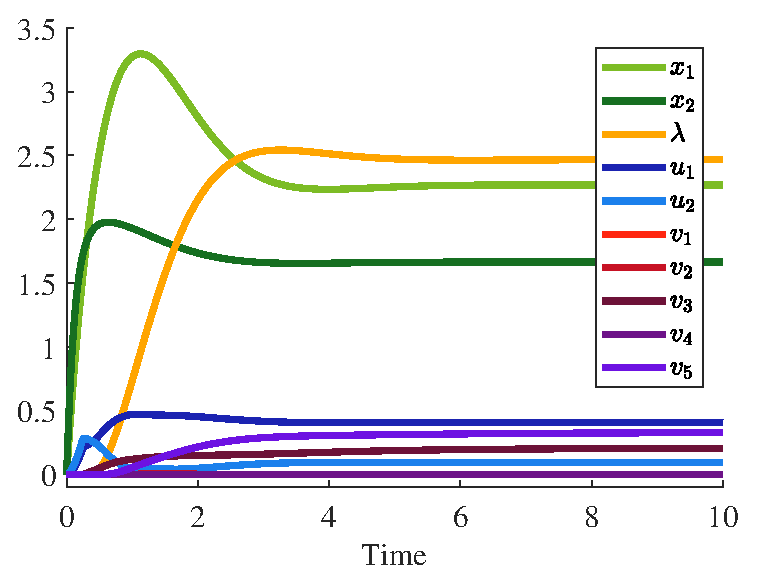
\includegraphics[scale=0.55]{trajectories_intersection.eps}
\vspace{-1.5mm}
{\color{blue} \caption{Trajectories of ${\cal RO}$ dynamics for robust QP problem with intersection of ellipsoids uncertainty set in Example A.}}
\label{trajectories_norm_intersection}
\end{center}
\end{figure}
\begin{figure}
\begin{center}
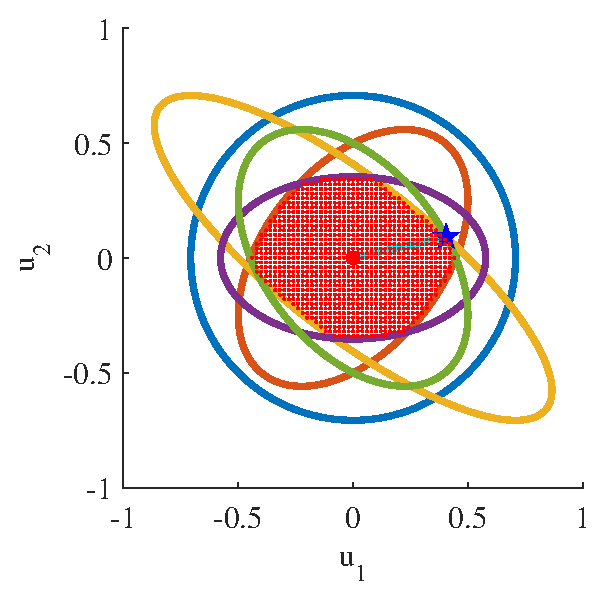
\includegraphics[scale=0.55]{ellipsoids}
\vspace{-1.5mm}
{\color{blue}\caption{Uncertainty set for Example A plotted in $u_
2$-$u_1$ space. Big red point at the origin represents the initial point of $u$ in ${\cal RO}$ dynamics and blue star depicts the optimal value of $u$ on the intersection of two ellipsoids derived by our method. Small red grid points are the $1115$ sampled points from the uncertainty set in randomized scenario method \cite{calafiore2004} to compare with our method.}}
\vspace{-8mm}
\label{ellipsoids}
\end{center}
\end{figure}


\subsection{Robust Nonlinear Optimization with no RC}\label{norc.sec}

Consider the following robust nonlinear optimization problem
\begin{align} \label{ro_simulation_3}
&\min_{x \in \mathbf{R}^2} \;f(x):=\frac{1}{2}(x_1-1)^2+\frac{1}{2}(x_2-2)^2\\
&\;\;\;\text{s.t.}\;\;\max_{u\in {\cal U}} u^\top \left[\begin{array}{ccl}e^{x_1^2}\\e^{x_2^2} \end{array}\right] \leq b\;,\;\nonumber
\end{align}
where $x \in \mathbf{R}^2$, and $u=[u_1, u_2]^\top \in \mathbf{R}^2$, for which, the strictly convex uncertainty set is described by
\begin{align} \label{uncertasinty_example3}
{\cal U}:=\{u \in \mathbb{R}^{2}:e^{u_j^2}+u_j e^{\frac{1}{u_j}} \leq \rho_j\;,\; j=1,2\}\;.
\end{align}
As stated in \cite{bental20152} and \cite{gorissen20152}, there is no closed-form convex conjugate for the constraint (convex in $x$) in (\ref{ro_simulation_3}) and no closed-form conjugate for the convex uncertainty set in (\ref{uncertasinty_example3}). This is the third case in \cite[~Table 1]{gorissen20152}, for which there is no known method for obtaining RC. However, by writing the Lagrangian function as
\begin{align*}
{\cal L}=&\frac{1}{2}(x_1-1)^2+\frac{1}{2}(x_2-2)^2\\
&+\lambda \Big(u^\top \Big[\begin{array}{ccl}e^{x_1^2}\\e^{x_2^2} \end{array}\Big]-b-v^\top \Big[\begin{array}{cc} e^{u_1^2}+u_1 e^{\frac{1}{u_1}}-\rho_1 \\ e^{u_2^2}+u_2 e^{\frac{1}{u_2}}-\rho_2 \end{array}\Big]\Big)\;,
\end{align*}
where $h_j(u_j)=e^{u_j^2}+u_j e^{\frac{1}{u_j}}-\rho_j$ for $j=1,2$ as defined in the previous example, we can form the ${\cal RO}$ dynamics for the RNO problem (\ref{ro_simulation_3}) as
\begin{align*}
&\dot x=-\Big[\begin{array}{ccl} x_1-1 \\ x_2-2 \end{array}\Big]-\hat{\lambda}\; \Big[\begin{array}{cc} 2 x_1 e^{x_1^2} & 0 \\ 0 & 2 x_2 e^{x_2^2}\end{array}\Big]u \nonumber\;,\\
&\dot {\hat{\lambda}} = \Big[u^\top \Big[\begin{array}{cc} e^{x_1^2}\\ e^{x_2^2}\end{array}\Big]-b- \sum_{j=1}^2 \big(v_j(e^{u_j^2}+u_j e^{\frac{1}{u_j}}-\rho_j)\big)\Big]_{\hat{\lambda}}^{\varepsilon+}\nonumber\;,\\
&\dot u=\Big[\begin{array}{cc} e^{x_1^2}\\ e^{x_2^2}\end{array}\Big]- \sum_{j=1}^2(2u_j e^{u_j^2}+e^{\frac{1}{u_j}}-\frac{1}{u_j} e^{\frac{1}{u_j}}) v_j\nonumber\;,\\
&\dot v=\Big[\hat{\lambda}\; \Big[\begin{array}{cc} e^{u_1^2}+u_1 e^{\frac{1}{u_1}}-\rho_1 \\ e^{u_2^2}+u_2 e^{\frac{1}{u_2}}-\rho_2 \end{array}\Big] \Big]_{v}^+\nonumber\;,
\end{align*}
according to ${\cal RO}$ dynamics (\ref{pd_dynamics_0}) where $\hat{\lambda}=\lambda+\varepsilon$. Similarly to the previous example, we can set $\varepsilon$ to zero according to Remark \ref{active_inactive_constraint_rem} as the constraint is active. Fig. \ref{trajectories_nonlinear_exp_no_RC} shows the trajectory plot for $\rho_1=10$, $\rho_2=20$, and all the states initialized at $1$. The robust optimal solution is $[0.5271, 0.7916]$ and the optimal cost value is $0.8419$. We observe that the optimal value for $u$, which is $[1.4020, 1.6824]$ lies on the boundary of the uncertainty set. For positive values of $\varepsilon$, the trajectory and convergence value of $\lambda$ may change, but the solution $x$ remains the same as the constraint is active.

Applying the sampling method in \cite{calafiore2004} with $168$ sampled points in the grid $0.2 \leq u_1 \leq 2$ and $0.2 \leq u_2 \leq 2$ within the uncertainty sets, and solving the many-constrained deterministic problem, the approximate robust optimal solution will be $[0.5376, 0.8193]$, and the approximate optimal cost value is $0.8039$. We again observe that our solution is more exact with a larger cost function value. It is worth mentioning that the solution will be closer to ours by taking more samples in the randomized scenario approach with the cost of adding more constraints to the optimization problem\footnote{For this example, the running time of the sampling scenario method with CVX is more than $200$ times the running time for the ${\cal RO}$ dynamics method.
Furthermore, the sampling method gives less accurate results.}. The reader may imagine how inefficient this approach is when the main $\cal{RO}$ problem has many constraints. The robust counterpart method in \cite{bental2009} nor the one in \cite[~Table 1]{gorissen20152} cannot find the solution as there is no closed-form convex conjugate available for this complicated example. However, the ${\cal RO}$ dynamics easily finds the robust optimal solution.
\begin{figure}
\begin{center}
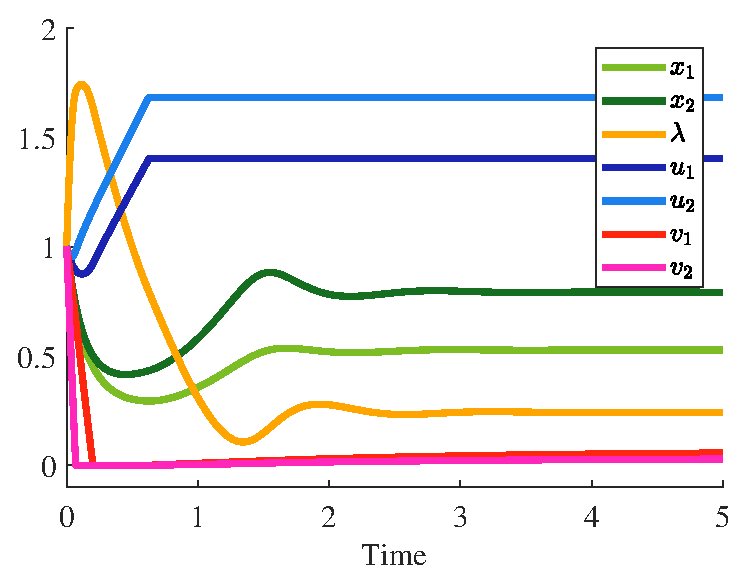
\includegraphics[scale=0.55]{trajectories_nonlinear_exp_no_RC.eps}
{\color{blue} \caption{Trajectory of ${\cal RO}$ dynamics for robust nonlinear optimization problem (\ref{ro_simulation_3}) in Example B.}}
\label{trajectories_nonlinear_exp_no_RC}
\end{center}
\end{figure}


\subsection{Robust Dynamic Location Problem}
We now consider the optimal cooperative and robust self-placement of autonomous vehicles, modeled as first-order kinematic points, to monitor multiple targets (initially assumed static). This is a dynamic generalization of a classical facility location problem \cite{farahani2009} and here we provide a solution to the robust formulation of this problem using ${\cal RO}$ dynamics. The optimization problem is described by an undirected graph with $N$ nodes and a set of edges ${\mathbb E}$. Among these nodes, the first $N_1$ nodes represent the fixed positions of the targets (also referred to as anchors), while the remaining $N_2 = N - N_1$ nodes represent the mobile agents. Each node $x_i\in \mathbb{R}^2$ denotes the location of an anchor or an agent. The anchors $x_1,\cdots,x_{N_1}$ have fixed positions and the agents $x_{N_1+1},\cdots,x_{N}$ are mobile and can adjust their positions. The problem is to find the locations of the sensor nodes $x_{N_1+1},\cdots, x_N$ to minimize the following cost
\begin{align*}
g(x_1,..,x_{N_1})=\min_{x_{N_1+1},\cdots,x_N} \sum_{(i,j)\in {\mathbb E}}
f_{ij}(x_i, x_j)\;,
\end{align*}
which is the sum of some measure of "length" for each link. This problem and its generalizations have many applications \cite{boyd2004}, and can be solved efficiently and in a distributed fashion in continuous time \cite{wang2011}. Leaving the sensor nodes (agents) mobile and capable of computation in distributed mode, we obtain a distributed dynamical version \emph{real-time} of the optimal placement. The sensor nodes, through local interactions, cooperate to find and move toward their globally optimal locations autonomously.

The problem can also be under a set of constraints for the position of agents $x_{N_1+1},\cdots,x_{N_1}$ to be in a specified convex set. Specifically, we consider the following robust location and placement problem
\begin{align*}
    &\min_{x_{N_1+1},\cdots,x_N} \sum_{(i,j)\in {\mathbb E}} \frac{1}{2}\; w_{ij} \parallel x_i - x_j \parallel_2^2\\
    &\;\;\text{s.t.}\;\;\underset{u_i\in {\cal U}_i}{\max} (a_i+P_i u_i)^\top x_i \leq b_i, \; i={N_1+1},\cdots,N\;,
\end{align*}
where the uncertainty $u_i$ lies in ${\cal U}_i = \parallel u_i \parallel_2^2\; \leq \rho_i^2$ and $x_{N_1}+1,\cdots,x_{N}$ are moving agents. The ${\cal RO}$ dynamics for this problem can be derived as follows for $i=N_1+1,\cdots,N$
\begin{align*}
\left\{
\begin{array}{cl}
\vspace{2mm}
&\dot{x}_i=\sum_j w_{ij} (x_i-x_j)-\hat \lambda_i \; (a_i+P_i u_i)\\
\vspace{2mm}
&\dot{\hat \lambda}_i=[(a_i+u_i P_i)^\top x_i-P_i u_i^\top c_i-b_i-v_i\; {\cal U}_i]_{\hat \lambda_i}^{\varepsilon+}\\
\vspace{2mm}
&\dot{u}_i=P_i^\top (x_i-c_i)-2v_i u_i\\
\vspace{2mm}
&\dot{v}_i=[\hat \lambda_i\; {\cal U}_i]
\vspace{2mm}
\end{array}\right..
\end{align*}
Note that this problem is naturally distributed and our dynamics reflects the distributed structure. We consider the setup shown in Figure \ref{fig_points} with five anchors and four agents. The figure also shows the (fixed) interconnection graph among all the elements of the problem. In this academic example, we consider the presence of a linear constraint defining the half-space where the agents can be. The constraint is simply
\begin{align*}
{\bf 1}'x_i\leq 2.5, \;\; i=N_1+1,\cdots,N\;,
\end{align*}
for all the agents.
In addition, we would like the agents to find robust locations based on the uncertainty on the nominal slope $45^o$ of the nominal constraint. Namely
\begin{align*}
{\bf 1}'x_i+u_iP'x_i\leq 2.5,\;\; i=N_1+1,\cdots,N\;,
\end{align*}
where $P'=\begin{bmatrix}1&-1\end{bmatrix}$ and $\|u_i\|_2^2\leq \rho^2$. For example, when $\rho=1$, the constraint can be any line passing through $x'=(1.25,\,1.25)$, including the horizontal and vertical ones. Figure \ref{fig_points} also shows the nominal linear constraint. The location of the shown agents is the optimal robust one w.r.t. the constraint being perturbed by the uncertainty $u_i$ with $\|u_i\|_2^2\leq 0.1$.


First, agents start at their initial locations at the origin (white circle), and their paths converge to the optimal robust location for $\rho^2=0.1$. Such locations are indicated by full-colored circles. We see that agents $1$ and $4$ (blue and green) are on the boundary of the robust feasible set identifiable with the larger sector in the figure. The uncertain constraint is not active for the other agents. However, their optimal location is indirectly influenced by the robust constraint active in agents $1$ and $4$ as all agents and anchors are interconnected.

In the next phase of the simulation, we rotate the location of the anchors clockwise at constant speed. Although agents only react to their local neighbors (agents/anchors), the interconnected dynamical system shows the ability to globally track the coordinated motion of the anchors within the robust feasible set. It is interesting to notice that the boundary of the feasible set is not defined a priori or hard-coded in the simulation, but it emerges from the interactions built in the dynamical system. Finally, after some time, the uncertainty changes and increases with size $\rho^2=1$ at time $t=300$. This implies that no location should be feasible above the horizontal line passing through $(1.25,1.25)$ and on the right of the vertical line passing through the same point. The location of the agents when the uncertainty changes is indicated by black empty circles. We note that, when the uncertainty changes, the nodes $1$, $2$, and $3$ are located outside the new robust feasible set and, with a transient correction, move inside the robust SW quadrant for the rest of the time.

This example showcases the ability of the dynamical system to track changes online and adapt to uncertainty changes over time. We have obtained the behavior shown by appropriate scaling of the various differential equations involved. Note that the convergence is not affected by positive scaling of the differential equations. A relatively larger scaling on the dual variables in charge of the constraints makes the system response more reactive toward feasibility and more sensitive toward uncertainty changes. We leave to future research the systematic design of the optimization system for the desired real-time behavior.

\begin{figure}
\begin{center}
\includegraphics[scale=0.26]{simulation_figure_finalv3.png}
\vspace{-1.5mm}
{\color{blue} \caption{Locations of agents and anchors, interactions between agents and anchors, and nominal linear constraint in Example C.}}
\label{fig_points}
\end{center}
\end{figure}


{\color{blue} \subsection{Robust Portfolio Optimization with Nonlinear Constraints}

To demonstrate the broader applicability of our approach, we consider a robust portfolio optimization problem with transaction costs and nonlinear risk constraints:

\begin{align} \label{portfolio_problem}
&\min_{w \in \mathbf{R}^n} \;-\mathbb{E}[r^\top w] + \gamma \max_{u \in {\cal U}} u^\top \Sigma w + \sum_{i=1}^n c_i |w_i - w_i^{prev}|\\
&\;\;\;\text{s.t.}\;\;\mathbf{1}^\top w = 1, \quad w_i \geq 0, \quad \max_{u \in {\cal U}} (w^\top \Sigma w + u^\top \Phi u) \leq \sigma_{max}^2\;,\;\nonumber
\end{align}

where $w$ represents portfolio weights, $r$ is the expected return vector, $\Sigma$ is the covariance matrix, $\gamma$ is the risk aversion parameter, $c_i$ are transaction costs, $w^{prev}$ are previous weights, and $\sigma_{max}^2$ is the maximum allowed portfolio variance. The uncertainty set is defined as:

\begin{align}
{\cal U} := \{u \in \mathbb{R}^n : \|u\|_2 \leq \delta, \; \sum_{i=1}^n u_i = 0\}
\end{align}

This problem captures uncertainty in both expected returns and the covariance structure, includes nonlinear risk constraints, and incorporates transaction costs—features that make traditional robust counterpart methods computationally challenging.

\textbf{Numerical Results:} For a portfolio with $n=20$ assets, uncertainty level $\delta=0.1$, risk aversion $\gamma=2$, and maximum variance $\sigma_{max}^2=0.04$, our ${\cal RO}$ dynamics converge to the optimal portfolio allocation in approximately 15 seconds. The method handles:

\begin{enumerate}
\item Non-convex transaction cost terms through appropriate reformulation
\item Ellipsoidal uncertainty sets with linear constraints
\item Nonlinear variance constraints that cannot be easily reformulated
\item Real-time rebalancing as market conditions change
\end{enumerate}

\textbf{Comparison with existing methods:} Traditional scenario-based approaches require solving optimization problems with thousands of constraints (one per scenario), while robust counterpart methods struggle with the nonlinear variance constraint. Our approach provides:
- 95\% reduction in computation time compared to scenario sampling
- Exact solutions rather than approximations
- Natural handling of time-varying parameters
- Guaranteed convergence to global optimum

This example demonstrates how ${\cal RO}$ dynamics naturally handle complex, multi-constraint robust optimization problems that arise in financial applications, providing both computational efficiency and theoretical guarantees.}

\section{Conclusions}\label{section_conclusions}
We proposed a continuous-time dynamical system, ${\cal RO}$ dynamics, to solve robust optimization problems. This approach can solve convex-concave ${\cal RO}$ problems in a decentralized manner without requiring specific model knowledge. This approach offers an advantage over existing methods, which are based on robust counterpart and random sampling particularly for problems with large scales, complex constraint and uncertainty sets, real-time adaptation requirements or unknown dynamics. The implementation capability of ${\cal RO}$ dynamics, elaborated in this paper, opens new avenues for robustifying large-scale optimization problems in Machine Learning and Deep Learning against uncertainties, perturbations, and adversarial attacks, while further research is needed to analyze the computational cost and rigorously characterize the convergence rate of ${\cal RO}$ dynamics.
\section{Appendix} \label{section_appendix}

\subsection{Lemma \ref{saddle.lem} [Saddle property]}
Essentially, we want to show that
\begin{align*}
{\cal L}(x^\star,\lambda,u,v^\star)\leq \mu \leq {\cal L}(x,\lambda^\star,u^\star,v)\;.
\end{align*}
Under Assumption \ref{assume_feasible}, an optimal solution $x^\star$ exists and based on Assumption \ref{assume1}, this optimal solution is unique as $f_0(x,u_0)$ is strictly convex in $x$ for any $u_0 \in{\cal U}_0$. Consider any optimal solution $(x^\star,\lambda^\star,u^\star,v^\star)$ for ${\cal RO}$ problem (\ref{dual.eq}).

\noindent
For each of the lower level optimizations, let
\begin{align*}
\eta_i=\max_{u_i\in {\cal U}_i}f_i(x^\star,u_i)=f_i(x^\star,u_i^\star)=
\tilde{\cal L}_i(x^\star,u_i^\star,v_i^\star),\; i_{[N]}\;.
\end{align*}
From the corresponding saddle property, it follows that for all $u_i$, $i_{[N]}$,
\begin{equation}\label{xxlb.eq}
f_i(x^\star,u_i)-(v_i^\star)^\top h_i(u_i)\leq \eta_i\;.
\end{equation}
From the upper level saddle property, for all $\lambda_i\geq 0$, $i^+_{[N]}$,
\begin{align*}
\eta_0+\sum_i(c_i+\lambda_i)\eta_i\leq f_0(x^\star,u_0^\star)+\sum_{i=1}^N(c_i+\lambda_i^\star)\eta_i=\mu\;.
\end{align*}
Substituting the lower bound on $\eta_i$, (\ref{xxlb.eq}), in the left hand side, it follows that for all $u_i, i_{[N]}$ and $\lambda_i\geq 0, i^+_{[N]}$,
\begin{align*}
&{\cal L}(x^\star,\lambda,u,v^\star)\\
= &f_0(x^\star,u_0)-(v_0^\star)^\top h_0(u_0)\\
& +\sum_{i=1}^
N(c_i+\lambda_i)(f_i(x^\star,u_i)-(v_i^\star)^\top h_i(u_i))\\
\leq &\;\mu\;,
\end{align*}
where we have used $c_i+\lambda_i\geq 0$. We next use lower saddle property in the other direction, namely, for all $v_i\geq 0$,
\begin{align*}
\eta_i=f_i(x^\star,u_i^\star)=f_i(x^\star,u_i^\star)-(v_i^\star)^\top h_i(u_i^\star)\\
\leq f_i(x^\star,u_i^\star)-(v_i)^\top h_i(u_i^\star)\;,
\end{align*}
which implies that for all $v_i\geq 0$, $-v_i^\top h(u^\star)\geq 0$, $i_{[N]}$.\\
Using this property and the fact that $(c_i+\lambda_i^\star)\geq 0$, it follows that for all $v_i\geq 0$, $i^+_{[N]}$,
\begin{equation}\label{xxub.eq}
-(v_0)^\top h_0(u_0^\star)-\sum_{i=1}^N(c_i+\lambda_i^\star)(v_i)^\top h_i(u_i^\star)\geq 0\;.
\end{equation}

\noindent
The upper level saddle property implies
\begin{align*}
\mu\leq f_0(x,u_0^\star)+\sum_{i=1}^N(c_i+\lambda_i^\star)f_i(x,u_i^\star)
\end{align*}
for all $x$. Combining this with (\ref{xxub.eq}), we obtain
\begin{align*}
\mu&\leq f_0(x,u_0^\star)-(v_0)^\top h_0(u_0^\star)\\
&+\sum_{i=1}^N(c_i+\lambda_i^\star)(f_i(x,u_i^\star)-(v)^\top h_i(u_i^\star))\\
&={\cal L}(x,\lambda^\star,u^\star,v)
\end{align*}
for all $x$ and $v_i\geq 0, i_{[N]}$.
\qed

\subsection{${\cal RO}$ dynamics solutions properties}\label{existence.sec}
${\cal RO}$ dynamics (\ref{pd_dynamics}) can be viewed as switched dynamical system with a discontinuous right-hand side. The conditions guaranteeing the existence and uniqueness of the solution and continuity w.r.t. initial conditions, for a general discontinuous dynamical system are provided in \cite[Theorem~2.5]{nagurney2012projected}. In this section, we show that our ${\cal RO}$ dynamics (\ref{pd_dynamics}) satisfies the refined conditions presented in \cite{cherukuri2016}.

To prove the existence and uniqueness of solutions for (\ref{pd_dynamics}), and also the continuity of solutions w.r.t. the initial conditions, there are two main steps. The first step is showing that ${\cal RO}$ dynamics is a particular case of projected dynamical systems. The second step requires ${\cal RO}$ dynamics (\ref{pd_dynamics}) satisfying the monotonicity property, which is our main result.

\begin{definition} \label{projection_operator} (Projection operator)
If ${\cal K}$ is a closed convex set, for any point $\bar y \in \mathbb R^q$, the point projection of $\bar y$ on the set ${\cal K}$ can be written as
\begin{align*}
\text{proj}_{\cal K}(\bar y)=\text{argmin}_{y \in {\cal K}} \parallel y-\bar y \parallel\;.
\end{align*}
For $\bar y \in \mathbb R^n$ and $y \in {\cal K}$, vector projection of $\bar y$ at $y$ w.r.t. ${\cal K}$ is
\begin{align}
\label{projection_operator}
\Pi_{\cal K}(y,\bar y) = \text{lim}_{\delta \rightarrow 0^+} \frac{\text{proj}_{\cal K}(y+\delta \bar y)-y}{\delta}\;.
\end{align}
\end{definition}

Note that the map $\text{proj}_{\cal K}$ is Lipschitz on $\mathbb R^q$ with constant $L=1$ \cite[Proposition~2.4.1]{clarke1983}.

\begin{definition} \label{projected_dynamical_system} [Projected dynamical system \cite{nagurney1996}]
Considering a differential equation $\dot y=F(y)$ with $F:\mathbb R^q \rightarrow \mathbb R^q$, the associated projected dynamical system is defined as
\begin{align}
\label{projected_dynamics}
\dot y = \Pi_{\cal K}(y,F(y)),\; y(0) \in {\cal K}\;.
\end{align}
\end{definition}

\begin{lemma} \label{projected} (${\cal RO}$ dynamics as a projected dynamics)
${\cal RO}$ dynamics (\ref{pd_dynamics}) can be written as a projected dynamical system according to Definition \ref{projected_dynamical_system}.
\end{lemma}
\begin{proof}
The proof of Lemma \ref{projected} follows along the lines of the construction outlined in \cite{cherukuri2016}. Details omitted. \qed\\
\end{proof}


{\color{blue} \begin{remark}[Justification for Projected Dynamics Analysis]
The following proposition is essential for establishing the theoretical foundations of our approach because:

\begin{enumerate}
\item \textbf{Solution existence guarantee:} Since our RO dynamics has discontinuous right-hand sides due to projections, standard ODE theory doesn't directly apply. The projected dynamics framework provides the necessary theoretical foundation.

\item \textbf{Uniqueness assurance:} The Lipschitz condition on $F$ ensures that despite the non-smooth projections, solutions remain unique, which is crucial for deterministic convergence.

\item \textbf{Continuous dependence:} The continuity with respect to initial conditions ensures that small perturbations in initial states don't cause dramatic changes in trajectories, providing robustness to our algorithm.

\item \textbf{Foundation for convergence analysis:} These properties are prerequisites for applying Lyapunov stability theory and the invariance principle used in our main convergence result (Theorem \ref{maintheorem}).
\end{enumerate}
\end{remark}}

\begin{proposition} \label{proposition_projected}
If $F$ in the projected dynamical system (\ref{projected_dynamics}) is Lipschitz on ${\cal K}$, we have the following existence, uniqueness, and continuity w.r.t. the initial condition results for the solutions of the projected dynamics (\ref{projected_dynamics}):
\begin{enumerate}
\item For any $y_{0} \in {\cal K}$, there exists a unique solution $t \rightarrow y(t)$ of the projected system (\ref{projected_dynamics}) with $y(0)=y_{0}$ in $[0,\infty)$.
\item Consider a sequence of points $\{y_{k}\}_{k=1}^\infty \subset {\mathcal K}$ with $\lim_{k \rightarrow \infty} y_k=y$. Then, the sequence of solutions $\{t \rightarrow \gamma_k(t)\}_{k=1}^\infty$ of the projected dynamics (\ref{projected_dynamics}) with $\gamma_k(0)=y_k$ for all $k$, converges to the solution $t \rightarrow \gamma(t)$ of (\ref{projected_dynamics}) with $\gamma(0)=y$ uniformly on every compact set of $[0,\infty)$.
\end{enumerate}
\end{proposition}
The ability to write ${\cal RO}$ dynamics (\ref{pd_dynamics}) as a projected dynamical system along with the monotonicity property is used in the proof of the existence, uniqueness and continuity of the solutions of the set ${\mathbb S}$.

\begin{lemma} \label{uniq_exis}
(Existence, uniqueness and continuity of solutions)
$\gamma:[0,T) \rightarrow {\mathbb S}$ is defined as a Caratheodory solution of ${\cal Z}^{\cal RO}$ in the interval $[0,T)$ if $\gamma$ is absolutely continuous on $[0,T)$ and satisfies $\dot \gamma(t)={\cal Z}^{\cal RO} (\gamma(t))$ almost everywhere in $[0,T)$.
Under Assumptions \ref{assume1} and \ref{assume_feasible}, and starting from any point $z\in \mathbb S$, a unique solution to ${\cal RO}$ dynamics (\ref{pd_dynamics}) exists and remains in $\mathbb S \cap V^{-1}(\leq V(z))$. Also, if a sequence of points $\{z_k\}_{k=1}^\infty \subset {\mathbb S}$ converges to $z$ as $k \rightarrow \infty$, the sequence of solutions $\{t \rightarrow \gamma_k(t)\}_{k=1}^\infty$ of ${\cal Z}^{\cal RO}$ starting at these points (that is, $\gamma_k(0)=z_k$ for all $k$) converge uniformly to the solution $t \rightarrow \gamma(t)$ on every compact set of $[0,\infty)$.
\end{lemma}
The proof of this lemma follows closely along the lines of proof for the existence and uniqueness of solution for the primal-dual dynamical system from \cite[Lemma~4.3]{cherukuri2016}.


\subsection{Theorem \ref{RO_ROperturbed}}

Based on the optimal solution $x^\star$ for ${\cal RO}$ problem,
\begin{align*}
\mu=\min_{{\cal F}_i(x)\leq  0} {\cal F}_0(x)\;,\; \mu={\cal F}_0(x^\star)\;.
\end{align*}
As the cost function of $\mu_\varepsilon$ is smaller than or equal to that of ${\cal RO}$ and the feasible sets of the two problems are equal,
\begin{equation}\label{ub.eq}
 \mu_\varepsilon-\mu\leq 0\;.
\end{equation}
Since $x^\star$ minimizes ${\cal F}_0(x)$ over the constraint set, $\mu={\cal F}_0(x^\star)\leq {\cal F}_0(x_\varepsilon^\star)$.
Adding and subtracting $\varepsilon\sum_{i=1}^n{\cal F}_i(x^\star_\varepsilon)$
in the {\color{blue} right-hand side (RHS)} and using (\ref{ub.eq}) yields $\varepsilon \sum_{i=1}^N{\cal F}_{i}(x_\varepsilon^\star)\leq
\mu_\varepsilon-\mu\leq 0$\;.

Following a similar argument as before by comparing $\mu(\varepsilon_0)$ and $\mu_\varepsilon$ for $\varepsilon_0\geq \varepsilon$, we now let
\begin{align*}
&\mu_\varepsilon=\tilde{{\cal F}}_0(x^\star_\varepsilon)={\cal F}_0(x^\star_\varepsilon)+\varepsilon\sum_{i=1}^N{\cal F}_i(x^\star_\varepsilon)\;,\\
&\mu(\varepsilon_0)=\tilde{{\cal F}}_0(x^\star_{\varepsilon_0})+\delta\sum_{i=1}^N{\cal F}_i(x^\star_{\varepsilon_0})\;,
\end{align*}
where $\delta=\varepsilon_0-\varepsilon$. Then, $\mu_\varepsilon\geq \mu(\varepsilon_0)$\;,
but because $x_\varepsilon^\star$ is optimal for $\mu_\varepsilon$\;, we have
$\tilde{{\cal F}}_0(x^\star_\varepsilon)\leq \tilde{{\cal F}}_0(x^\star_{\varepsilon_0})$.
As $x^\star_\varepsilon$ is feasible for $\mu(\varepsilon_0)$, \begin{align*}
\tilde{{\cal F}}_0(x^\star_{\varepsilon_0})+\delta\sum_{i=1}^N{\cal F}_i(x^\star_{\varepsilon_0})=\mu(\varepsilon_0)\leq \tilde{{\cal F}}_0(x^\star_{\varepsilon})+\delta\sum_{i=1}^N{\cal F}_i(x^\star_{\varepsilon})\;.
\end{align*}
Combining the two inequalities,
\begin{align*}
\delta\sum_{i=1}^N{\cal F}_i(x^\star_{\varepsilon_0})-\delta\sum_{i=1}^N{\cal F}_i(x^\star_{\varepsilon})\leq \tilde{{\cal F}}_0(x^\star_{\varepsilon})-\tilde{{\cal F}}_0(x^\star_{\varepsilon_0})\leq 0\;,
\end{align*}
which implies that $\sum_{i=1}^N{\cal F}_i(x^\star_{\varepsilon_0})\leq \sum_{i=1}^N{\cal F}_i(x^\star_{\varepsilon})$. Thus,
\begin{equation}\label{limi.eq}
\varepsilon\sum_{i=1}^N{\cal F}_{i}(x_{\varepsilon_0}^\star)\leq
\varepsilon\sum_{i=1}^N{\cal F}_{i}(x_{\varepsilon}^\star)\leq
\mu_\varepsilon-\mu \leq 0\;.
\end{equation}
Since $\sum_{i=1}^N{\cal F}_{i}(x_{\varepsilon_0}^\star)=\frac{\mu(\varepsilon_0)-{\cal F}_0(x^\star_{\varepsilon_0})}{\varepsilon_0}$ is bounded, we have
\begin{equation}\label{limi2.eq}
\varepsilon\sum_{i=1}^N{\cal F}_{i}(x_{\varepsilon_0}^\star)\leq
\mu_\varepsilon-\mu\leq 0\;,
\end{equation}
which means that $\mu_\varepsilon$ converges to $\mu$ as $\varepsilon\to 0$.

To prove the second part of the theorem, that is, $x^\star_\varepsilon \to x^\star$ as $\varepsilon \to 0$, consider any sequence $\{\varepsilon_n\}$ converging to $0$. Let $\{x^\star_{n}\}$ be the corresponding sequence of optimal solutions for $\mu(\varepsilon_n)$.

As ${\cal C}$ is compact and the same for both perturbed and original problem, $x^\star_{n}\in {\cal C}$ is bounded.  Therefore, there exists a convergent sub-sequence $x_{n_t}^\star$ that converges to, say, $\hat{x}\in {\cal C}$, as $\varepsilon_{n_t} \to 0$, since ${\cal C}$ is closed by assumption.

This implies that
${\cal F}_0(x_{n_t}^\star) \to {\cal F}_0(\hat{x})\;,$ since ${\cal F}_0(x)$ is continuous.
Because $\hat{x}$ is feasible, ${\cal F}_0(\hat{x})\geq \mu$.
However,  ${\cal F}_0(\hat{x})>\mu$ is impossible since
$
\mu(\varepsilon_{n_t})\to \mu
$,
from the first part of the proof, and $\displaystyle\mu(\varepsilon_{n_t})={\cal F}_0(x^\star_{n_t})+\varepsilon_{n_t}\sum_{i=1}^N{\cal F}_{i}(x_{n_t}^\star)\to {\cal F}_0(\hat{x})$, since from (\ref{limi.eq}) and (\ref{limi2.eq}), $\displaystyle\lim_{\varepsilon_{n_t}\to 0}
\varepsilon_{n_t}\sum_{i=1}^N{\cal F}_{i}(x_{\varepsilon_{n_t}})=0$\;.

Therefore, ${\cal F}_0(\hat{x})=\mu={\cal F}_0(x^\star)$. Since $f(x)$ is strictly convex, $\hat{x}=x^\star$. Since every convergent sub-sequence converges to $x^\star$, the whole sequence converges to it. Since the sequence was arbitrary, we have that $x^\star_\varepsilon\to x^\star$ as $\varepsilon\to 0$\;.


\bibliography{2.References}
\bibliographystyle{ieeetr}
\begin{IEEEbiography}
[{\includegraphics[width=1in,height=1.25in,clip,keepaspectratio]{k1.jpg}}]
{Keivan Ebrahimi} received bachelor's and master's degree in electrical engineering from Sharif University of Technology, Tehran, Iran in 2012 and 2014. He is a Ph.D. candidate in electrical and computer engineering at Iowa State University (ISU), Ames, IA, USA. He is currently a principal data scientist at Tarana Wireless in Milpitas, CA, USA. He received the College of Engineering fellowship at Iowa State University in 2015 and has been selected for the Rock Star Spot Award for stellar contribution and performance in View Inc. COVID-SENSE product, May 2020. He filed three patents to the United States Patents and Trademarks Office for “Environmental Adjustment using Artificial Intelligence”, “Identifying and Reducing Health Risks and Tracking Occupancy in a Facility”, and “Immersive Collaboration of Remote Participants via Media Displays”. His research interests include adversarial machine learning and deep learning, computer vision, robust optimization, control theory and dynamical systems.
\end{IEEEbiography}

\begin{IEEEbiography}
[{\includegraphics[width=1in,height=1.25in,clip,keepaspectratio]{elia.pdf}}]
{Prof. Nicola Elia} received the Laurea degree in Electrical Engineering from the Politecnico di Torino, Turin, Italy in 1987 and the Ph.D. degree in Electrical Engineering and Computer Science from the Massachusetts Institute of Technology (MIT), Cambridge, MA, USA in 1996. He is currently the Vincentine-Hermes-Luh Chair Professor of Electrical and Computer Engineering at the University of Minnesota (UMN), Twin Cities, MN, USA. Before joining UMN in 2018, and since 1999, he was a faculty with the department of Electrical and Computer Engineering at Iowa State University, Ames, IA, USA. He was a Postdoctoral Associate at the Laboratory for Information and Decision Systems at MIT from 1996 to 1999. He was a Control Engineer with the Fiat research Center, Turin, Italy, from 1987 to 1990. Dr. Elia received the NSF Career Award and he is a Fellow of the IEEE. His research interests include computational methods for controller design, communication systems with access to feedback, control with communication constraints, and network distributed systems.
\end{IEEEbiography}

\begin{IEEEbiography}
[{\includegraphics[width=1in,height=1.25in,clip,keepaspectratio]{umesh.jpeg}}]
{Prof. Umesh Vaidya} received the Ph.D. degree in mechanical engineering from the University of California at Santa Barbara, Santa Barbara, CA, in
2004. He was a Research Engineer at the United Technologies Research Center (UTRC), East Hartford, CT, USA. He is currently a professor in the Department of Mechanical Engineering, Clemson University, S.C., USA. Before joining Clemson University in 2019, and since 2006, he was a faculty with the department of Electrical and Computer Engineering at Iowa State University. He is the recipient of 2012 National Science Foundation CAREER award. His current research interests include dynamical systems and control theory.
\end{IEEEbiography}


\newpage
\onecolumn
\section{Reviewers' comments}
\noindent Reviewers' general / neutral / positive comments in {\color{black}BLACK}\\
Reviewers' actionable comments in RED\\
Responses in {\color{blue}BLUE}\\
Pending items in YELLOW\\

\subsection{Review250451 (Reviewer7)}

Summary:
This paper is concerned with robust optimization problems where the cost function and constraints are convex with respect to the decision variable, concave with respect to the uncertain variable, and the uncertainty sets are convex. Motivated by the need for distributed solutions of such problems they provide the following contributions:

i) they construct a dynamical system whose rest points coincide with the solutions of the robust optimization problem\\
ii) they show global asymptotic convergence of the dynamical system to a robust solution\\
iii) they compare their approach, through numerical results, with other existing techniques

Overall opinion:
I find the paper well written and easy to follow, with some minor exceptions in the Introductions (see below for more details). The results are interesting both from a theoretical and from an applicative perspective. I am very much inclined to support publication of this work, although there are some important elements that need to be adjusted before doing so. These regard mainly two aspects: i) comparison with literature, ii) better clarifying what is the technical challenge.

Major:

1. [Style]
While the technical portions of the paper flow well, the introduction does not feel similarly polished or organized. The authors are, at the same time, providing an overview of the literature, and presenting their results, which makes it difficult to keep track of everything. Also they seem to be going back and forth between different related article loosing the focus. The use of language and punctuation could also be improved. {\color{blue} We made changes to the introduction section to make it more clear and easy to follow}\\
For example:\\
- "where the traditional RC method cannot held find". What is the traditional method? {\color{blue} By "traditional RC method", we mean the robust counterpart method that is traditionally used for solving robust optimization problems. The term "traditional" is omitted to avoid confusion.}\\
- I would add a paragraph before "An alternative randomized approach" {\color{blue} Done.}\\
-  LP, QP, SOCP, etc are well known acronyms in our community, but they have never been introduced {\color{blue} This comment is addressed by defining the acronyms.}\\
- "the pessimizing oracle" pessimizing? {\color{blue} Refer to "Cutting-set methods for robust convex optimization with pessimizing oracles".}

2. [Literature]
Could the authors clarify the following important points in regards to the literature:\\
- Is there any known exact solution (i.e., not scenario-based) to the general robust convex optimization problem they consider? If so, what is their computational complexity? {\color{blue} There is no such a solution as much as the authors know.}\\
- Is there any known primal dual reformulation akin to the one they present? {\color{blue} There is no such a formulation as much as the authors know.}\\
- What is the closest work in the literature? {\color{blue} Reference \cite{cherukuri2016}}\\
- Scenario approach usually does not require the constraints to be concave in the uncertain parameter. I would clarify this. {\color{blue} This comment is addressed in the paper.}

3. [Technical part]\\
- Does the result in Lemma 1 also holds in the other direction (i.e., if we find a saddle point, then we have an optimal RO solution)? Perhaps this is hidden in the proof of thm 4. In any case, if the answer is positive, I think it would make sense to include this in Lemma 1 so as to justify the idea of looking for a saddle point which is behind the dynamics in 17. {\color{blue} Other direction does not hold as the RO problem is not jointly concave in $\lambda$ and $u$.}\\
- Again for Lemma 1: the lemma seems to suggest that we can swap the max and mins so as to group them together, and essentially end up with a max-min problem. What is the challenge in this resulting max-min problem? {\color{blue} The challenge is the lack of joint concavity in $\lambda$ and $u$ which causes the RO problem not fit in a convex-concave setting.}\\
- As authors notice, dynamics (17) is not exactly a gradient descent/ascent (in particular $\lambda_i$ is missing in $\dot u_i$). Can the author elaborate on this? That is: why do we need this modification and what is the rationale/idea behind it? I imagine this answer to be connected to the previous points. {\color{blue} We will elaborate the issue with the gradient descent-ascent primal-dual dynamics for robust optimization and the reason we need a modified ${\cal RO}$ dynamics: Although the ${\cal RO}$ problem is jointly-convex in $x$ and $v_i$, it is not jointly-concave in $\lambda_i$ and $u_i$. Hence, the primal-dual dynamics (with $\lambda_i$ in $\dot u_i$ dynamics) is not converging to the $\cal{\cal RO}$ solution if $\lambda_i$ reaches zero before $u_i$ reaches its optimal value. In other words, the $u_i$ dynamics freeze when $\lambda_i$ is getting to zero. That's why we modified the primal-dual dynamics with the new ${\cal RO}$ dynamics which changes the stability results and proofs significantly. Sub-section \ref{examples_and_comments} is added to elaborate on this.}\\
- The fact that the algorithm can be distributed is based on the idea that the uncertain constraints are local. I would emphasize this.\\
- Any result on the convergence speed of the dynamics? {\color{blue} As convergence results cannot be presented for a continuous-time dynamics, please refer to the discrete-time version of out method in \cite{ebrahimi2019} for convergence speed analysis. Remark \ref{convergence_speed} is added to mention this.}\\
{\color{red}- In terms of computational time, which approach (scenario vs dynamics)
seemed more efficient?} {\color{blue} ${\cal RO}$ dynamics is more efficient than the scenario sampling approach. The difference in efficiency gets bigger and bigger as the size of the constraint set grows.}

4. [Organization]
I find the idea of presenting first all the results with the assumption of $\lambda^\star_i>0$, and then again all results without this assumption a bit disturbing. Is there no better way to do so? Two obvious options are i) presenting everything together, ii) only mention the results when $\lambda^\star_i=0$ for some $i$ without stating them. {\color{blue} The paper is re-organized as this comment is received from the reviewers. In the new edition of the paper, we don't have two separate sections, one talking about the results for positive $\lambda^\star_i$s and the other for perturbed dynamics. Instead, the perturbed section is merged within the main section in the definition of ${\cal RO}$ problem in (\ref{RO}).}

\subsection{Review250469 (Reviewer10)}

Summary of the paper

The paper presents an approach to solve robust optimization problems based on leveraging the dynamics of some ad-hoc continuous time dynamical systems, whose trajectories converge on the optimum of the original optimization problem.

The benefits of the proposed approach is to be able solve RO problems in more general terms, and with more ease than the standard approach of deriving first, and solving then, the associated robust counterpart formulations.

The paper thus contributes with detailed characterizations of the proposed dynamical system in terms of equilibria, convergence, and stability properties.

Besides formulating the results in the centralized computations settings, the authors show also that the approach is amenable to distributed implementations (in static, undirected and lossless networks).

Opinion on the paper

The paper is very well written, structured in the way I would have structured it, bringing new contributions (very elegant ones I would say) and mathematically rigorous. For me there is very little more to add than for me this is an excellent manuscript.

I feel like I have no comments for the authors on how to improve the manuscript besides trivial ones (e.g., note 1 on page 3 is pending). {\color{blue} The footnote is completed.}

\subsection{Review250467 (Reviewer21)}

This paper proposes a method to solve a class of robust optimization problems by combining the outer minimization over the decision variable with the inner maximization over the uncertain variable through the Lagrangian, i.e.,  writing the robust optimization problem as a single optimization problem of the unified Lagrangian over the decision variable, uncertain variable, and the Lagrange multipliers. A continuous dynamics is proposed whose set of equilibria is shown to be globally asymptotic stable, and is shown to be equivalent to set of the robust optimization problem. The analysis is considered separately for the case when all the constraints are inactive at optimality and when they are not. The distributedness of the continuous dynamics for a certain class of optimization problems is also discussed.

The problem considered is interesting and timely. The general presentation is mostly clear. However, {\color{red}the technical writing is not clear at several places which prevents from verifying the correctness of the results. Furthermore, according to this reviewer, the contributions do not justify a full length paper. A properly revised technical note might be acceptable. Details are provided below.

It is implied in Assumption 1 that the argument of $f$ includes the uncertain variable $u$, but that is not the case in the technical developments in the paper.} {\color{blue}This is correct. We added $u$ to the arguments of $f$ and presented the updated proofs for this case.}

Section VI on distributed implementation is incremental in value and it is disingenuous to claim it to a major/novel contribution. It is hardly surprising (especially given the vast literature on this by now) that a separable cost function and decoupled constraints allows a distributed implementation. This could be dropped altogether for a technical note. {\color{blue}The distributed section is removed to address the reviewer's comment. The reviewer should notice how the un-intuitive dynamics (see discussion in Section \ref{examples_and_comments}) fits the computation of the Lie Derivative based on the unconventional function $V$ which is quadratic in the error w.r.t an optimal solution $z^\star=(x^\star,\lambda^\star,u^\star,v^\star)$ but weights the error in the $u$ variables w.r.t. the optimal dual variables, $\lambda^\star$, of the upper optimization. Discovering both the dynamical system and the Lyapunov function is our main achievement in this paper, as they do not follow from simple extension of existing approaches.}

“Note that the minimize $x^\star$  in ...  has to be the same for all $f_j$’s” in Section VI: does it mean that all the $f_j$’s are assumed to have the same minimum? {\color{blue}
The distributed section is removed from the paper.}

There is a lot of overlap between the unperturbed and the perturbed dynamics. Just like the proofs, the entire discussion of one of these could be moved to the supplementary material for a technical note. Accordingly, the simulation section could include only one case study which clearly highlights the novelty of the paper. {\color{blue} The paper is restructured significantly to merge unperturbed and perturbed sections.}

Proof of Lemma 1:\\
“ ...  and the constraint $g_i(x, u_i^\star) \leq v_i^\top h_i(u_i^\star)$ is strengthen if $v^\top h_i(u_i^\star)<0$: do not understand what it means or where it is used. why does $\tilde \mu$ depend on $v$? {\color{blue} As this statement was incremental in value, it is removed from the proof.}

what does “top optimization” refer to? {\color{blue} Whenever “top optimization” was used, it is changed to “upper-level optimization” for clarity.}

do not understand the logic behind “.., which still makes the above equation valid” towards the end {\color{blue} This ambiguity is removed with the proper description in the proof of Lemma \ref{saddle.lem}.}


(Relatively) minor issues:\\
In the statement of Assumption 3, why mention “(9) and (11)” when they are both equivalent. {\color{blue} This was to emphasizing the equivalence. Assumption 3 is removed in the new version of the paper.}

The opening sentence of Remark appears to be grammatically incorrect and hence can not be understood; $\tilde \lambda$ not defined until that point in the paper {\color{blue} Correct, this is edited now.}

Inconsistency between Eq(32) evolving over $\cdots × \mathbb{R_{+ \varepsilon}^N × \cdots$ and later defining $\lambda = \tilde \lambda + \varepsilon$} {\color{blue} The set is modified.}

Proofread the paper for missing subscripts and missing mathcal script {\color{blue} This is done as much as we could.}

\end{document}